%% 
%% Copyright 2019-2024 Elsevier Ltd
%% 
%% This file is part of the 'CAS Bundle'.
%% --------------------------------------
%% 
%% It may be distributed under the conditions of the LaTeX Project Public
%% License, either version 1.3c of this license or (at your option) any
%% later version.  The latest version of this license is in
%%    http://www.latex-project.org/lppl.txt
%% and version 1.3c or later is part of all distributions of LaTeX
%% version 1999/12/01 or later.
%% 
%% The list of all files belonging to the 'CAS Bundle' is
%% given in the file `manifest.txt'.
%% 
%% Template article for cas-sc documentclass for 
%% double column output.

\documentclass[a4paper,fleqn,numbers]{cas-sc}

% If the frontmatter runs over more than one page
% use the longmktitle option.

%\documentclass[a4paper,fleqn,longmktitle]{cas-sc}

\usepackage[numbers]{natbib}
%\usepackage[authoryear]{natbib}
%\usepackage[authoryear,longnamesfirst]{natbib}
\usepackage{amsmath,amssymb,amsfonts}
\usepackage{amsthm}
\usepackage{tikz}
\usepackage{geometry}
\usepackage{graphicx}
\usepackage{enumitem}
\usepackage{subcaption}
\usepackage{float}
\usepackage{caption}
\usepackage{booktabs}
\usepackage{listings}
\usepackage{xcolor}
%%%Author macros
\def\tsc#1{\csdef{#1}{\textsc{\lowercase{#1}}\xspace}}
\tsc{WGM}
\tsc{QE}
%%%

% Uncomment and use as if needed
\newtheorem{theorem}{Theorem}[section]
\newtheorem{definition}[theorem]{Definition}
\newtheorem{lemma}[theorem]{Lemma}
\newtheorem{corollary}[theorem]{Corollary}
\newtheorem{proposition}[theorem]{Proposition}
\newtheorem{example}[theorem]{Example}
\newtheorem*{remark}{Remark}
%\newdefinition{rmk}{Remark}
%\newproof{pf}{Proof}
%\newproof{pot}{Proof of Theorem \ref{thm}}

\DeclareMathOperator{\Head}{Head}
\DeclareMathOperator{\Tail}{Tail}
\DeclareMathOperator{\Sop}{S}

\begin{document}
	\let\WriteBookmarks\relax
	\def\floatpagepagefraction{1}
	\def\textpagefraction{.001}
	\let\printorcid\relax    
	
	% Short title
	\shorttitle{}    
	
	% Short author
	\shortauthors{}  
	
	% Main title of the paper
	\title [mode = title]{Research on the Denominator-Weighted Shapiro Cyclic Sum and Efficient Solution Algorithms}
	
	% Title footnote mark
	% eg: \tnotemark[1]
	\tnotemark[1] 
	
	% Title footnote 1.
	% eg: \tnotetext[1]{Title footnote text}
	\tnotetext[1]{This work was supported by the Tongji University Student Innovation Training Program (SITP) under No. X2025634.} 
	
	% First author
	%
	% Options: Use if required
	% eg: \author[1,3]{Author Name}[type=editor,
	%       style=chinese,
	%       auid=000,
	%       bioid=1,
	%       prefix=Sir,
	%       orcid=0000-0000-0000-0000,
	%       facebook=<facebook id>,
	%       twitter=<twitter id>,
	%       linkedin=<linkedin id>,
	%       gplus=<gplus id>]
	
	\author[1]{Anqi Wang}%[<options>]
	
	% Footnote of the first author
	\fnmark[1]
	
	% Email id of the first author
	\ead{wang_anqi@tongji.edu.cn}
	
	% URL of the first author
	%\ead[url]{}
	
	% Credit authorship
	% eg: \credit{Conceptualization of this study, Methodology, Software}
	\credit{}
	
	% Address/affiliation
	
	%\author[1]{William {J. Hansen}}%[]
	
	%\cormark[1]
	% Footnote of the second author
	
	% Corresponding author indication
	%\fnmark[2]
	
	% Email id of the second author
	%\ead{wjh@example.org}
	
	% URL of the second author
	%\ead[url]{}
	
	% Credit authorship
	\credit{}
	
	% Address/affiliation
	\affiliation[1]{organization={School of Mathematical Sciences, Tongji University},
		city={Shanghai},
		postcode={200092}, 
		country={China}}
	
	% Corresponding author text
	\cortext[2]{Corresponding author}
	
	% Footnote text
	\fntext[1]{}
	
	% For a title note without a number/mark
	\nonumnote{}
	
	% Here goes the abstract
	\begin{abstract}
		This paper investigates the extremal properties and solution strategies of the \textbf{denominator-weighted Shapiro cyclic sum}. First, the fundamental properties of the \textbf{Shapiro cyclic sum} are derived, the structural characteristics and piecewise patterns of the minimizer of this cyclic sum are explored, and a general method for deriving the minimum of this cyclic sum is presented. To address the issue of extremely complex algebraic computations in high-dimensional cases, this paper transforms the constrained optimization problem into a Riemannian manifold optimization problem on the unit sphere through variable substitution, and proposes an efficient \textbf{Riemannian BFGS (RBFGS) algorithm} equipped with an oscillatory solution detection and restart mechanism. Numerical experiments demonstrate that the proposed algorithm exhibits good convergence and efficiency in verifying counterexamples to the classical Shapiro inequality and solving for the minimum of its denominator-weighted form.
	\end{abstract}
	
	% Use if graphical abstract is present
	%\begin{graphicalabstract}
	%\includegraphics{}
	%\end{graphicalabstract}
	
	% Research highlights
	\begin{highlights}
		\item Establishes key properties and characteristic results of the denominator-weighted Shapiro cyclic sum.
		
		\item Extends the Bushell–Ando structural characterization of minimizers to the denominator-weighted case.
		
		\item Reduces the minimization problem to solving finitely many polynomial equation systems.
		
		\item An efficient RBFGS algorithm on the unit sphere is proposed to minimize the Shapiro cyclic sum.
	\end{highlights}
	
	
	% Keywords
	% Each keyword is seperated by \sep
	\begin{keywords}
		Shapiro inequality\sep Shapiro cyclic sum\sep Riemannian BFGS algorithm\sep Minimizer analysis\sep
	\end{keywords}
	
	\maketitle
	
	% Main text
	\section{Introduction}\label{}
	
	Cyclic inequality is a classical inequality with an elegant structure and a wide range of applications, see\cite{steele2004}. In 1954, Shapiro proposed the following famous cyclic inequality: for $n(n\geq 3)$ nonnegative real numbers $x_1, x_2, \ldots, x_n$,
	\[
	\sum_{i=1}^{n} \frac{x_i}{x_{i+1}+x_{i+2}} \geq \frac{n}{2},
	\tag{1.1}
	\]
	where $x_{n+1}=x_1$ and $x_{n+2}=x_2$.
	
	This problem underwent exploration for over thirty years until it was completely resolved by Troesch in 1989: the inequality holds when $n$ is even and $4 \leq n \leq 12$, or when $n$ is odd and $3 \leq n \leq 23$; counterexamples exist when $n$ is even and $n \geq 14$, or when $n$ is odd and $n \geq 25$, see\cite{troesch1985}\cite{troesch1989}. Subsequently, scholars such as Bushell, Ando, and others further investigated the conditions for equality when the inequality holds, see\cite{bushell1994}\cite{bushell2002}\cite{ando2013}.
	
	To broaden the theoretical depth and application scope, attention has turned to various generalizations of the Shapiro inequality. See, e.g.,  \cite{choudhury2022}\cite{radulescu2012}\cite{tanriverdi2012}. Nguyen and Le \cite{nguyen2009} systematically studied the following denominator-weighted Shapiro inequality:
	\[
	\sum_{i=1}^{n} \frac{x_i}{p x_{i+1} + q x_{i+2}} \geq \frac{n}{p+q},
	\tag{1.2}
	\]
	where $p,q \geq 0$ and $p+q>0$. Clearly, both sides of the denominator-weighted Shapiro inequality are homogeneous with respect to $p+q$, so one may assume $p+q=1$ without loss of generality. In particular, when $p=q=1/2$, (1.2) reduces to the classical Shapiro inequality (1.1). Nguyen and Le proved that (1.2) always holds for $n=3$; for $n=4$, (1.2) holds if and only if $p \geq q$, i.e., under $p+q=1$ the necessary and sufficient condition is $\frac{1}{2}\leq p \leq 1$; for $n=5$, a sufficient condition for the inequality to hold is $\dfrac{5-\sqrt{5}}{10} \leq p \leq \dfrac{5+\sqrt{5}}{10}$; when $n$ is even and $0\leq p<\frac{1}{2}$, (1.2) never holds. 
	
	In Section 3 of this paper, we will analyze further properties of the denominator-weighted Shapiro inequality, and based on Ando's analysis of the structure of minimizers of the classical Shapiro cyclic sum, systematically extend his method to the denominator-weighted case, summarizing a general approach for finding the minimum point and minimum value of the Shapiro cyclic sum for a given integer $n$ and weight $p$. To overcome the difficulty of analytical solution for relatively large $n$, Section 4 further proposes a BFGS algorithm based on Riemannian manifolds, providing theoretical characterization and numerical tools for the study of the minimum of the denominator-weighted Shapiro cyclic sum and the Shapiro inequality problem.
	
	\section{Preliminaries}\label{}
	
	\subsection{Known Results of Shapiro Cyclic Sum and Shapiro Inequality in the Denominator-Weighted Form}
	
	For an $n$-dimensional vector $x=(x_1,x_2,\cdots,x_n)\in \mathbb{R}^n$ and weight $p$, denote the denominator-weighted Shapiro cyclic sum by
	\[
	F(x,p)=\sum_{i=1}^{n} \frac{x_i}{px_{i+1}+qx_{i+2}}.
	\tag{2.1}	
	\]
	Then the denominator-weighted Shapiro inequality is
	\[
	F(x,p)=\sum_{i=1}^{n} \frac{x_i}{px_{i+1}+qx_{i+2}}\geq n,
	\tag{2.2}
	\]
	where $x=(x_1,x_2,\cdots x_n)$, $x_i\geq 0$, $p+q=1$, $0\leq p \leq 1$, $x_{n+1}=x_1$, $x_{n+2}=x_2$.
	
	In particular, when $p=\frac{1}{2}$, (2.1) and (2.2) reduce to the classical Shapiro cyclic sum and inequality, respectively, i.e.,
	\[
	F\left(x,\frac{1}{2}\right)=\sum_{i=1}^{n} \frac{x_i}{\frac{1}{2} x_{i+1}+\frac{1}{2}x_{i+2}}\geq n.
	\]
	
	Note that by continuity, when the denominators are nonzero, there is no difference in studying whether the inequality holds on the domain $x_i\geq 0$ or $x_i > 0$. To facilitate the study of the minimum of the cyclic sum, we set $x_i\geq 0$ in the following.
	
	\begin{theorem}
		For the classical Shapiro inequality, the following hold:
		\begin{enumerate}
			\item If $n$ is odd and $3 \leq n \leq 23$, then
			\[
			F\left(x,\frac{1}{2}\right)=\sum_{i=1}^{n} \frac{x_i}{\frac{1}{2} x_{i+1}+\frac{1}{2}x_{i+2}}\geq n.
			\]
			Furthermore, equality $F\left(x,\frac{1}{2}\right) = n$ holds if and only if $x_1 = x_2 = \cdots = x_n$.
			\item If $n$ is even and $4 \leq n \leq 12$, then
			\[
			F\left(x,\frac{1}{2}\right)=\sum_{i=1}^{n} \frac{x_i}{\frac{1}{2} x_{i+1}+\frac{1}{2}x_{i+2}}\geq n.
			\]
			Furthermore, equality holds if and only if $x$ is of oscillatory type, i.e., there exist $a>0,b>0$ such that $(x_1,\cdots,x_n) = (a,b,a,b,\cdots,a,b)$.
			\item If $n$ is even and $n \geq 14$, or $n$ is odd and $n \geq 25$, then there exist $x_1>0,\ldots,x_n>0$ such that $F\left(x,\frac{1}{2}\right)<n$.
		\end{enumerate}
	\end{theorem}
	
	\begin{theorem}[Nguyen, Le, 2009]
		\begin{enumerate}
			\item When $n=3$, for any $0\leq p\leq 1$, $F(x,p) \geq 3$ always holds.
			\item When $n=4$, the inequality $F(x,p) \geq 4$ always holds if and only if $\frac{1}{2}\leq p \leq 1$.
			\item When $n=5$, a sufficient condition for the inequality $F(x,p) \geq 5$ to always hold is $\frac{5-\sqrt5}{10} \leq p \leq \frac{5+\sqrt5}{10}$.
			\item If $n \geq 4$ is even and $0\leq p < \frac{1}{2}$, then there exists $x=(x_1,\dots,x_n) > 0$ such that $F(x,p)< n$, i.e., the inequality does not hold.
		\end{enumerate}
	\end{theorem}
	
	\subsection{BFGS Algorithm}
	
	There are many tools in numerical computation for optimization problems, such as rank-one update formula, BFGS formula, DFP formula, etc., among which the BFGS formula is the most widely used, see \cite{chen2005}.
	
	%Consider the unconstrained problem
	%\[
	%\min f(x) , x\in \mathbb{R}^n,
	%\]
	%where the function $f:\mathbb{R}^n\to \mathbb{R}$ has continuous first-order partial derivatives.
	%Stationary points of $f$, i.e., points $x\in\mathbb{R}^n$ where $\nabla f(x)=0$, are necessary conditions for extreme points. Therefore we need to focus on the zeros of the equation $\nabla f(x)=0$. Since $\nabla f:\mathbb{R}^n\to\mathbb{R}^n$ is continuous, finding stationary points can be related to solving systems of nonlinear equations. We need to approximate the Jacobian matrix of $\nabla f$, which is the Hessian matrix of $f$. Let
	%\[
	%x^{(k+1)} = x^{(k)} + \lambda_k d^{(k)},
	%\]
	%where $d^{(k)}$ is the \textbf{search direction} at $x^{(k)}$,
	%\[
	%d^{(k)} = -\nabla^2 f(x^{(k)})^{-1} \nabla f(x^{(k)}),
	%\]
	%and $\lambda_k=1$ or the optimal step size from $x^{(k)}$ along the search direction. We aim to construct an approximation matrix $H_k$ to $\nabla^2 f(x^{(k)})^{-1}$.
	%\[
	%f(x) \approx f(x^{(k+1)}) + \nabla f(x^{(k+1)})^T (x - x^{(k+1)}) + \frac{1}{2} (x - x^{(k+1)})^T \nabla^2 f(x^{(k+1)}) (x - x^{(k+1)}),
	%\]
	%\[
	%\nabla f(x) \approx \nabla f(x^{(k+1)}) + \nabla^2 f(x^{(k+1)}) (x - x^{(k+1)}).
	%\]
	%Setting $x = x^{(k)}$, we have
	%\[
	%\nabla f(x^{(k)}) \approx \nabla f(x^{(k+1)}) + \nabla^2 f(x^{(k+1)}) (x^{(k)} - x^{(k+1)}).
	%\]
	%Denote $s^{(k)} = x^{(k+1)} - x^{(k)}$, $y^{(k)} = \nabla f(x^{(k+1)}) - \nabla f(x^{(k)})$, then
	%\[
	%y^{(k)} \approx \nabla^2 f(x^{(k+1)}) s^{(k)}.
	%\]
	%Assuming the Hessian matrix $\nabla^2 f(x^{(k+1)})$ is invertible, we have
	%\[
	%s^{(k)} \approx \nabla^2 f(x^{(k+1)})^{-1} y^{(k)}.
	%\]
	
	%We replace the inverse Hessian matrix $\nabla^2 f(x^{(k+1)})^{-1}$ in the above expression with a matrix $H_{k+1}$ that does not involve second-order derivative calculations, and require $H_{k+1}$ to satisfy
	%\[
	%s^{(k)} = H_{k+1} y^{(k)}.
	%\]
	%This equation is the quasi-Newton equation. We can update $H_{k+1}$ using methods such as rank-one update formula, BFGS formula, DFP formula, etc., among which the BFGS formula is the most widely used, see \cite{chen2005}.
	
	\begin{theorem}[BFGS formula for optimization problems] 
		The BFGS formula for constructing the approximation matrix $H_k$ to $\nabla^2 f(x^{(k)})^{-1}$ is given by:
		\[
		H_{k+1} = \left(I - \frac{s^{(k)} y^{(k)T}}{y^{(k)T} s^{(k)}} \right) H_k \left(I - \frac{y^{(k)} s^{(k)T}}{y^{(k)T} s^{(k)}} \right) + \frac{s^{(k)} s^{(k)T}}{y^{(k)T} s^{(k)}},
		\]
		or equivalently:
		\[
		H_{k+1} = H_k +\frac{s^{(k)} s^{(k)T}}{y^{(k)T} s^{(k)}} +  \frac{y^{(k)T} H_k y^{(k)} s^{(k)} s^{(k)T}}{(y^{(k)T} s^{(k)})^2} - \frac{s^{(k)} y^{(k)T} H_k + H_k y^{(k)} s^{(k)T}}{y^{(k)T} s^{(k)}}.
		\]
	\end{theorem}
	
	The BFGS algorithm for the unconstrained optimization problem $\min\limits_{x \in \mathbb{R}^n} f(x)$ ($f\in C^1$) proceeds as follows:
	
	\begin{enumerate}
		\item Initialization: Choose an initial point $x^{(0)} \in \mathbb{R}^n$, set $H_0 = I_{n}$.
		\item For $k = 0,1,2,\ldots$, perform:
		\begin{enumerate}
			\item Compute the gradient $g^{(k)} = \nabla f(x^{(k)})$. If $\|g^{(k)}\| < \varepsilon$ (where $\varepsilon$ is a preset tolerance) or the maximum number of iterations is exceeded, output $x^{(k)}$ and terminate.
			\item Compute the search direction $d^{(k)} = -H_k g^{(k)}$.
			\item Determine the step size $\lambda_k$ via a line search satisfying the Wolfe conditions.
			\item Update the point: $x^{(k+1)} = x^{(k)} + \lambda_k d^{(k)}$.
			\item Compute the difference vectors:
			\[
			s^{(k)} = x^{(k+1)} - x^{(k)}, \quad
			y^{(k)} = \nabla f(x^{(k+1)}) - \nabla f(x^{(k)}).
			\]
			\item Update the inverse Hessian approximation using the BFGS formula:
			\[
			H_{k+1} = \left(I - \frac{s^{(k)} y^{(k)T}}{y^{(k)T} s^{(k)}} \right) H_k \left(I - \frac{y^{(k)} s^{(k)T}}{y^{(k)T} s^{(k)}} \right) + \frac{s^{(k)} s^{(k)T}}{y^{(k)T} s^{(k)}}.
			\]
		\end{enumerate}
	\end{enumerate}
	
	%\begin{remark}[Wolfe line search conditions]
		
%		Let the current iterate be $x^{(k)}$, and suppose the search direction $d^{(k)}$ satisfies $\nabla f(x^{(k)})^{T} d^{(k)} < 0$ (descent direction). The step size $\lambda > 0$ must satisfy the following two conditions simultaneously:
%		
%		\begin{enumerate}
%			\item \textbf{Armijo condition (sufficient decrease condition)}:
%			\[
%			f(x^{(k)} + \lambda d^{(k)}) \leq f(x^{(k)}) + c_1 \lambda \, \nabla f(x^{(k)})^{T} d^{(k)},
%			\]
%			where $c_1 \in (0,1)$ is a constant.
%			\item \textbf{Curvature condition}:
%			\[
%			\nabla f(x^{(k)} + \lambda d^{(k)})^{T} d^{(k)} \geq c_2 \, \nabla f(x^{(k)})^{T} d^{(k)},
%			\]
%			where $c_2 \in (c_1, 1)$ is a constant.
%		\end{enumerate}
		
	%\end{remark}
	
%	\begin{lemma}
%		If $\nabla f(x^{(k)})\neq 0$ and $H_0=I_n$, then the matrices $H_k$ constructed by the BFGS algorithm are all symmetric positive definite.
%	\end{lemma}
%	
%	\begin{proof}
%		We use mathematical induction. When $k=0$, $H_0 = I_n$, which is clearly symmetric positive definite. Assume that for $k$, $H_k$ is symmetric positive definite. For $H_{k+1}$, the BFGS update formula is
%		\[
%		H_{k+1} = \left(I - \frac{s^{(k)} y^{(k)T}}{y^{(k)T} s^{(k)}} \right) H_k \left(I - \frac{y^{(k)} s^{(k)T}}{y^{(k)T} s^{(k)}} \right) + \frac{s^{(k)} s^{(k)T}}{y^{(k)T} s^{(k)}}.
%		\]
%		Set $A = I - \dfrac{s^{(k)} y^{(k)T}}{y^{(k)T} s^{(k)}}$, then $A^T = I - \dfrac{y^{(k)} s^{(k)T}}{y^{(k)T} s^{(k)}}$, and therefore
%		\[
%		H_{k+1} = A H_k A^T + \frac{s^{(k)} s^{(k)T}}{y^{(k)T} s^{(k)}}.
%		\]
%		Since $H_k$ is symmetric, $A H_k A^T$ is symmetric, and $\dfrac{s^{(k)} s^{(k)T}}{y^{(k)T} s^{(k)}}$ is symmetric, it follows that $H_{k+1}$ is symmetric.
%		
%		To prove positive definiteness, by the Wolfe conditions in Newton and quasi-Newton methods, we have $\langle y^{(k)}, s^{(k)} \rangle = y^{(k)T} s^{(k)} > 0$. For any nonzero vector $v \in \mathbb{R}^n$, consider the quadratic form:
%		\[
%		v^T H_{k+1} v = v^T A H_k A^T v + v^T \frac{s^{(k)} s^{(k)T}}{y^{(k)T} s^{(k)}} v.
%		\]
%		Let $u = A^T v$, then $v^T A H_k A^T v = u^T H_k u$, and
%		\[
%		v^T \frac{s^{(k)} s^{(k)T}}{y^{(k)T} s^{(k)}} v = \frac{(v^T s^{(k)})^2}{y^{(k)T} s^{(k)}}.
%		\]
%		Thus,
%		\[
%		v^T H_{k+1} v = u^T H_k u + \frac{(v^T s^{(k)})^2}{y^{(k)T} s^{(k)}}.
%		\]
%		Since $H_k$ is positive definite, $u^T H_k u \geq 0$; and because $y^{(k)T} s^{(k)} > 0$, we also have $\dfrac{(v^T s^{(k)})^2}{y^{(k)T} s^{(k)}} \geq 0$.
%		
%		If $v^T H_{k+1} v = 0$, then $u^T H_k u = 0$ and $(v^T s^{(k)})^2 = 0$. From $u^T H_k u = 0$ and the positive definiteness of $H_k$, we obtain $u = 0$, i.e.,
%		\[
%		A^T v = 0 \implies \left(I - \frac{y^{(k)} s^{(k)T}}{y^{(k)T} s^{(k)}}\right) v = 0.
%		\]
%		Hence $v = \dfrac{y^{(k)} s^{(k)T} v}{y^{(k)T} s^{(k)}}$. Let $\beta = \dfrac{s^{(k)T} v}{y^{(k)T} s^{(k)}}$, then $v = \beta y^{(k)}$. From $(v^T s^{(k)})^2 = 0$ we get $(\beta y^{(k)T} s^{(k)})^2 = 0$. Since $y^{(k)T} s^{(k)} > 0$, it follows that $\beta = 0$, and consequently $v = 0$. Therefore, for any nonzero $v$, $v^T H_{k+1} v > 0$, i.e., $H_{k+1}$ is positive definite.
%		
%		By mathematical induction, $H_k$ is symmetric positive definite for all $k \geq 1$.
%	\end{proof}
%	
%	\begin{theorem}[Convergence of the BFGS algorithm]
%		If $f$ is a twice continuously differentiable real function on $\mathbb{R}^n$ and satisfies (the strong convexity condition) that for any $\hat{x} \in \mathbb{R}^n$, there exists a constant $m > 0$ such that for all $x \in C(\hat{x}) = \{ x \mid f(x) \leqslant f(\hat{x}) \}$ and for all $y \in \mathbb{R}^n$,
%		\[
%		m\ \| y \|^2 \leqslant y^{\mathrm{T}} \nabla^2 f(x)  y,
%		\]
%		then the sequence $\{x^{(k)}\}$ generated by the BFGS algorithm either terminates at or converges to the unique minimizer of $f$ on $\mathbb{R}^n$.
%	\end{theorem}
%	
%	\begin{remark}
%		The proof of this theorem and related theoretical extensions can be found in the book \textit{Unconstrained Optimization Computation} by Professor Deng Naiyang\cite{deng1982}.
%	\end{remark}
	
	\section{Minimum of the Denominator-Weighted Shapiro Cyclic Sum}
	
	\subsection{Notation and Basic Properties}
	
	For the denominator-weighted Shapiro cyclic sum
	\[
	F(x,p)=\sum_{i=1}^{n} \frac{x_i}{px_{i+1}+qx_{i+2}},
	\]
	where $x=(x_1,x_2,\cdots x_n)$, $x_i\geq 0$, $p+q=1$, $0\leq p \leq 1$, $x_{n+1}=x_1$, $x_{n+2}=x_2$. Denote
	\begin{align*}
		\partial_i F(x,p) &= \frac{\partial}{\partial x_i} F(x,p) = \frac{1}{px_{i+1}+qx_{i+2}} - \frac{qx_{i-2}}{(px_{i-1}+qx_i)^2} - \frac{px_{i-1}}{(px_i+qx_{i+1})^2}, \\
		\partial_p F(x,p) &= \frac{\partial}{\partial p} F(x,p) = \sum_{i=1}^{n} \frac{x_i (x_{i+2} - x_{i+1})}{(px_{i+1} + qx_{i+2})^2}, \\
		\overline{K}_n &:= \{(x_1, \cdots, x_n) \in \mathbb{R}^n \mid x_1 \geq 0, \ldots, x_n \geq 0\}, \\
		K_n^\circ &:= \{(x_1, \cdots, x_n) \in \mathbb{R}^n \mid x_1 > 0, \ldots, x_n > 0\}, \\
		K_n^{\bullet} &:= \{(x_1, \cdots, x_n) \in \overline{K}_n \mid (x_1, \ldots, x_n) \notin K_n^{\circ}, (x_i, x_{i+1}) \neq (0,0),\forall i =1,2,\ldots,n\}, \\
		K_n &:= K_n^\circ \cup K_n^{\bullet}, \\
		P(n,p) &:=\inf\limits_{x \in K_n} F(x,p).
	\end{align*}
	
	By the AM-GM inequality, we have
	\[
	P(n,0)=\inf\limits_{x \in K_n} F(x,0)=\inf\limits_{x \in K_n} \sum_{i=1}^{n} \frac{x_i}{x_{i+2}}=n,\quad
	P(n,1)=\inf\limits_{x \in K_n} F(x,1)=\inf\limits_{x \in K_n} \sum_{i=1}^{n} \frac{x_i}{x_{i+1}}=n.
	\]
	
	Furthermore, taking $x=(1,1,\cdots,1)$, we have $F(x,p)=n$, so $P(n,p)\leq n$.
	
	\begin{theorem}[Existence of the minimum]
		For any integer $n\geq 3$ and $0<p<1$, there exists $x \in K_n$ such that $P(n,p)=F(x,p)$.
	\end{theorem}
	
	\begin{proof}
		Note that \(F(x, p)\) is homogeneous of degree zero: for any \(t > 0\), \(F(tx, p) = F(x, p)\). Therefore, we consider the domain as the set \(\{ x \in K_n \mid \sum_{i=1}^n x_i = 1 \}=S\cap K_n\), where $S= \{ x \in \mathbb{R}^n \mid x_i \geq 0, \sum_{i=1}^n x_i = 1 \}$, which is compact. he proof is then completed by this compactness. 
	\end{proof}
	
%	\begin{proof}
%		Note that \(F(x, p)\) is homogeneous of degree zero: for any \(t > 0\), \(F(tx, p) = F(x, p)\). Therefore, we consider the domain as the set \(\{ x \in K_n \mid \sum_{i=1}^n x_i = 1 \}=S\cap K_n\), where $S= \{ x \in \mathbb{R}^n \mid x_i \geq 0, \sum_{i=1}^n x_i = 1 \}$, which is compact.
%		
%		Take a minimizing sequence \(\{x^{(m)}\} \subseteq S \cap K_n\) such that \(F(x^{(m)}, p) \to P(n, p)\). Since \(S\) is compact, there exists a convergent subsequence \(\{x^{(m_k)}\}\) converging to some point \(x^* \in S\). We now show that \(x^* \in K_n\).
%		
%		If not, i.e., \(x^* \notin K_n\), then there exists some \(i\) such that \(x_i^* = x_{i+1}^* = 0\). Since \(\sum_{i=1}^n x_i^* = 1\), there exists some \(j\) such that \(x_j^* > 0\). Then there exists $j$ such that $x_j^* > 0$ and $x_{j+1}^*=x_{j+2}^*=0$. For the subsequence \(x^{(m_k)}\), when \(k\) is sufficiently large, we have \(x_j^{(m_k)} \to x_j^* > 0\), \(x_{j+1}^{(m_k)} \to x_{j+1}^*=0\), and \(x_{j+2}^{(m_k)} \to x_{j+2}^*=0\). The term \(\frac{x_j^{(m_k)}}{p x_{j+1}^{(m_k)} + q x_{j+2}^{(m_k)}}\) has denominator tending to zero and numerator tending to a positive number, hence this term tends to infinity, causing \(F(x^{(m_k)}, p) \to \infty\), which contradicts \(F(x^{(m_k)}, p) \to P(n, p) \leq n\).
%		
%		Therefore, \(x^*\in S\cap K_n\) is a minimizer, and the minimum exists.
%	\end{proof}
	
	\begin{theorem}
		\begin{enumerate}
			\item $P(n+2,p)\leq P(n,p)+
			\begin{cases} 
				\dfrac{1}{1-p}, & \text{if } p > \dfrac{1}{2}, \\ 
				2, & \text{if } p \leq \dfrac{1}{2}.
			\end{cases}$
			\item For odd $n\geq 3$, $P(n+1,p)\leq P(n,p)+1$.
		\end{enumerate}
	\end{theorem}
	
	\begin{proof}
		(1) Suppose $P(n,p)=F(x^*,p)$ with $x^*=(x_1,x_2,\cdots,x_n)\in K_n$. Considering $x'=(x_1,x_2,\cdots,x_n,x_1,x_2)\in K_{n+2}$, the proof becomes quite simple. 
		
%		(1) Suppose $P(n,p)=F(x^*,p)$ with $x^*=(x_1,x_2,\cdots,x_n)\in K_n$. Consider $x'=(x_1,x_2,\cdots,x_n,x_1,x_2)\in K_{n+2}$. Then
%		\begin{align*}
%			P(n+2,p)\leq F(x',p)&=\sum_{i=1}^{n} \frac{x_i}{p x_{i+1}+q x_{i+2}} 
%			+ \frac{x_1}{p x_2 + q x_1} 
%			+ \frac{x_2}{p x_1 + q x_2}\\
%			&=P(n,p)+\frac{x_1}{p x_2 + q x_1} 
%			+ \frac{x_2}{p x_1 + q x_2}\\
%			&\leq P(n,p)+
%			\begin{cases} 
%				\dfrac{1}{1-p}, & \text{if } p > \dfrac{1}{2}, \\ 
%				2, & \text{if } p \leq \dfrac{1}{2}.
%			\end{cases}
%		\end{align*}
		
		(2) Suppose $P(n,p)=F(x^*,p)$ with $x^*=(x_1,x_2,\cdots,x_n)\in K_n$. Consider $x^r=(x_1,x_2,\cdots,x_{r-1},x_r,x_r,x_{r+1},\cdots,x_n)\in K_{n+1}$. Then
		\begin{align*}
			F(x^r,p)-F(x^*,p)-1&=\frac{x_{r-1}}{px_r + qx_r}+\frac{x_r}{px_r + qx_{r+1}}-\frac{x_{r-1}}{px_r+ x_{r+1}} -1 = \frac{q(x_r -x_{r-1})(x_r -x_{r+1})}{px_r^2 + qx_r x_{r+1}}
		\end{align*}
		
		If there exists $r$ such that $(x_r -x_{r-1})(x_r -x_{r+1})\leq 0$, then we obtain
		\[
		P(n+1,p)\leq F(x^r,p)\leq F(x^*,p)+1=P(n,p)+1.
		\]
		
		Otherwise, if for all $r$, $(x_r -x_{r-1})(x_r -x_{r+1}) > 0$, then
		\[
		\prod_{r=1}^n (x_r-x_{r+1})^2 = \prod_{r=1}^n (x_{r-1}-x_r)(x_r-x_{r+1}) < 0,
		\]
		a contradiction.
	\end{proof}
	
	\begin{theorem}
		$P(n,p)$ is a continuous function of $p \in (0,1)$.
	\end{theorem}
	
	\begin{proof}
		Consider the domain as the set \(\{ x \in K_n \mid \sum_{i=1}^n x_i = 1 \}=S\cap K_n\), where $S= \{ x \in \mathbb{R}^n \mid x_i \geq 0, \sum_i x_i = 1 \}$, which is compact.
		
		Fix $n$ and $p_0$. There exists $x^*\in S\cap K_n$ such that $F(x^*,p_0)=P(n,p_0)$. For this $x^*$, there exists $\epsilon_0 >0$ such that for all $i$, $x_i$ and $x_{i+1}$ are not both $<\epsilon_0$. Denote $T_n^i(\epsilon)=\{x\in \mathbb{R}^n\mid x_i <\epsilon,x_{i+1}<\epsilon\}$. Then for any $0<\epsilon \leq \epsilon_0$, $x^*\in A(\epsilon)=S\setminus\cup_{i=1}^n T_n^i(\epsilon)\subseteq S\cap K_n$, where $A(\epsilon)=S\setminus\cup_{i=1}^n T_n^i(\epsilon)$ is always compact.
		
		If there exist $0<\epsilon\leq\epsilon_0$ and $\delta > 0$ such that for all $p\in (p_0 -\delta,p_0 +\delta)\cap (0,1)$, $F(x,p)$ attains its minimum at some $x^p \in A(\epsilon)=S\setminus\cup_{i=1}^n T_n^i(\epsilon)$, then by Berge's Maximum Theorem, considering $F(x,p)$ as a continuous function on a compact set $ A(\epsilon) \times [p_0 - \delta/2 , p_0 + \delta/2] $, where $A(\epsilon)$ does not change with $p$ within a small range, the value function $P(n,p) = \min\limits_{x \in A(\epsilon)} F(x, p)$ is a continuous function of the parameter $p$.
	\end{proof}
	
	\begin{lemma}
		There exist $\epsilon>0$ and $\delta > 0$ such that for all $p\in (p_0 -\delta,p_0 +\delta)\cap (0,1)$, $F(x,p)$ attains its minimum at some $x^p \in A=S\setminus\bigcup_{i=1}^n T_n^i(\epsilon)$.
	\end{lemma}
	
	\begin{proof}
		Suppose otherwise. For any sequences $\epsilon_k \to 0$ and $\delta_k \to 0$ ($k =1,2,\ldots$), there exist a sequence of parameters $p_k$ and a corresponding sequence of minimizers $x^{(k)}$ satisfying:
		\begin{itemize}
			\item $|p_k - p_0| < \delta_k$, i.e., $p_k \to p_0$.
			\item $x^{(k)}$ is a minimizer of $F(x, p_k)$ on $S \cap K_n$, and $x^{(k)} \in S\cap(\cup_{i=1}^n T_n^i(\epsilon_k))$. 
			That is, for each $k$, there exists some index $j_k$ such that $x_{j_k}^{(k)} < \epsilon_k$ and $x_{j_k+1}^{(k)} < \epsilon_k$.
		\end{itemize}
		Since $S$ is compact in $\mathbb{R}^n$, the sequence $\{x^{(k)}\}$ must have a convergent subsequence. Without loss of generality, denote this convergent subsequence by $\{x^{(k)}\}$ and let its limit be $x^{**} \in S$, i.e., $x^{(k)} \to x^{**}\in S$ as $k \to +\infty$.
		
		For each $k$, there exists an index $j_k$ such that two consecutive components are less than $\epsilon_k$. Since there are only $n$ indices (finitely many), there must exist some index $j$ such that $j_k = j$ infinitely often in the subsequence. Consider this subsequence and assume $x_j^{(k)} < \epsilon_k$ and $x_{j+1}^{(k)} < \epsilon_k$ for all $k$. Taking the limit $k \to +\infty$, by sign preservation we have
		\[
		x_j^{**} = 0 \quad \text{and} \quad x_{j+1}^{**} = 0.
		\]
		
		If $x_{j-1}^{**}> 0$, then the term $\frac{x_{j-1}^k}{p_k x_j^k +q_k x_{i+1}^k}$ in $\{F(x_k,p_k)\}_k$ tends to $+\infty$, a contradiction.
		
		If $x_{j-1}^{**}=0$, proceeding inductively backward, and considering $x^{**}\in S$, we again obtain a contradiction.
	\end{proof}
	
	\begin{definition}
		We say that $x=(x_1, \cdots, x_n) \in K_n$ and $y=(y_1, \cdots, y_n) \in K_n$ have the same pattern if $x_i=0 \Leftrightarrow y_i=0$ for all $i=1, \ldots, n$.
		
		Let $x=(x_1, \cdots, x_n) \in {K}_n^{\bullet}$. If $x_{i} = 0$, $x_{i+1}\neq 0, \ldots, x_{i+l}\neq0$, and $x_{i+l+1} = 0$, where $i,l \geq 1$, then $(x_{i+1}, \cdots, x_{i+l})$ is called a segment of $x$, and $l$ is called the length of this segment.
		
		For a segment $s:=(x_i, \cdots, x_j)$ of $x$, we denote
		\[
		\Sop(s) := \sum_{k=i}^{j-1} \frac{x_k}{p x_{k+1}+q x_{k+2}}, \quad \text{Head}(s) := x_i, \quad \text{Tail}(s) := x_j.
		\]
		Here, if the length of $s$ is $1$, then $\Sop(s)=0$.
		
		Let $s_1, \ldots, s_r$ be all segments of $x$. Let $l_k$ be the length of $s_k$. The tuple $(l_1, \cdots, l_r)$ is called the pattern of $x$. We have
		\[
		F(x,p) = \sum_{k=1}^r \Sop(s_k) + \sum_{k=1}^r \frac{\Tail(s_{k-1})}{q\Head(s_k)},
		\]
		where we adopt the convention $s_{k+r}=s_k$ for $k \in \mathbb{Z}$, and the indices of segments are periodic with period $r$.
	\end{definition}
	
	\begin{theorem}
		Assume that $P(n,p)=\min\limits_{x \in K_n^{\bullet}} F(x,p) = F(x^* ,p)$ is attained at $x^*\in K_n^{\bullet}$. Let $s_1, \ldots, s_r$ be all segments of $x^*$ (arranged in order), and let $l_k$ be the length of $s_k$. Then the following conclusions hold.
		
		\begin{enumerate}
			\item $\frac{\Tail(s_1)}{\Head(s_2)} = \frac{\Tail(s_2)}{\Head(s_3)} = \cdots = \frac{\Tail(s_{r-1})}{\Head(s_r)} = \frac{\Tail(s_r)}{\Head(s_1)}$.
			\item Assume $ x^* = (s_1, 0, s_2, 0, \cdots, s_r, 0) $, and let $\sigma$ be a permutation of $ \{1,2,\dots,r\} $. Then there exist positive real numbers $ t_1, t_2, \dots, t_r > 0 $ such that the vector $ x' = (t_1 s_{\sigma(1)}, 0, t_2 s_{\sigma(2)}, 0, \cdots, t_r s_{\sigma(r)}, 0) $ satisfies $F(x',p) = F(x^*,p) $.
		\end{enumerate}
	\end{theorem}
	
	The proof follows the same lines as Theorem 2.4 in \cite{ando2013}.
	
%	\begin{proof}
%		Since \( F(x,p) \) is invariant under cyclic shifts, we may cyclically shift appropriately so that $ x^*= (s_1, 0, s_2, 0, \cdots, s_r, 0) $. Denote $ x_k = \operatorname{Head}(s_k) $ and $ y_k = \operatorname{Tail}(s_k) $. Then
%		\[
%		F(x^*,p) = \sum_{k=1}^r \Sop(s_k) + \sum_{k=1}^r \frac{y_{k-1}}{q x_k},
%		\]
%		where indices are taken modulo $ r $, i.e., $ y_0 = y_r $, $ x_{r+1} = x_1 $. Here $ \Sop(s_k) = \sum\limits_{i \in s_k \text{ interior}} \frac{x_i}{p x_{i+1} + q x_{i+2}} $.
%		
%		(1) Consider a segment-wise scaling transformation: for each $ k=1,2,\ldots,r $, take $ t_k > 0 $ and define the vector
%		\[
%		x' = (t_1 s_1, 0, t_2 s_2, 0, \cdots, t_r s_r, 0).
%		\]
%		Then
%		\[
%		F(x',p) = \sum_{k=1}^r \Sop(s_k) + \sum_{k=1}^r \frac{t_{k-1} y_{k-1}}{q t_k x_k}.
%		\]
%		By the AM-GM inequality,
%		\[
%		\sum_{k=1}^r \frac{t_{k-1} y_{k-1}}{q t_k x_k} \geq r \cdot \left( \prod_{k=1}^r \frac{t_{k-1} y_{k-1}}{q t_k x_k} \right)^{1/r} = r \cdot \frac{1}{q} \left( \prod_{k=1}^r \frac{y_{k-1}}{x_k} \right)^{1/r},
%		\]
%		with equality if and only if all terms $ \frac{t_{k-1} y_{k-1}}{t_k x_k} $ are equal. There exists a choice of $ t_k $ making these terms equal; for example, set $ t_1 = 1 $ and define recursively $ t_j = \frac{y_1 \cdots y_{j-1}}{x_2 \cdots x_j} \cdot \left( \frac{x_1 \cdots x_r}{y_1 \cdots y_r} \right)^{(j-1)/r} $. Then $ F(x',p) $ attains this lower bound. Since $ x^* $ is a minimizer, corresponding to $ t_1 = \cdots = t_r = 1 $, we must have $ F(x^*,p) \leq \min\limits_{t_k >0} F(x',p) \leq F(x^*,p) $, so equality must hold. Hence when $ t_k = 1 $ the above inequality is an equality, implying that all terms $ \frac{y_{k-1}}{x_k} $ are equal, i.e.,
%		\[
%		\frac{y_1}{x_2} = \frac{y_2}{x_3} = \cdots = \frac{y_r}{x_1}.
%		\]
%		Thus
%		\[
%		\frac{\Tail(s_1)}{\Head(s_2)} = \frac{\Tail(s_2)}{\Head(s_3)} = \cdots = \frac{\Tail(s_{r-1})}{\Head(s_r)} = \frac{\Tail(s_r)}{\Head(s_1)}.
%		\]
%		
%		(2) Given a permutation $ \sigma $, let $ R = \left( \prod_{k=1}^r \frac{y_k}{x_k} \right)^{1/r} $. From (1), we have $ \frac{y_{k-1}}{x_k} = R $ for all $ k $. Similarly, there exist $ t'_1, \dots, t'_r > 0 $ such that for all $ k $,
%		\[
%		\frac{t'_{\sigma(k-1)} y_{\sigma(k-1)}}{q t'_{\sigma(k)} x_{\sigma(k)}} = \frac{1}{q} R.
%		\]
%		We can set $ t'_{\sigma(1)} = 1 $ and then define recursively $ t'_{\sigma(k)} = \frac{y_{\sigma(k-1)}}{R x_{\sigma(k)}} t'_{\sigma(k-1)} $. For the resulting $ x' = (t'_1 s_{\sigma(1)}, 0, t'_2 s_{\sigma(2)}, 0, \cdots, t'_r s_{\sigma(r)}, 0) $, we have
%		\[
%		F(x',p) = \sum_{k=1}^r \Sop(s_k) + \sum_{k=1}^r \frac{t'_{\sigma(k-1)} y_{\sigma(k-1)}}{q t'_{\sigma(k)} x_{\sigma(k)}} = \sum_{k=1}^r \Sop(s_k) + r \cdot \frac{1}{q} R = F(x^* ,p).
%		\]
%	\end{proof}
	
	\begin{corollary}
		For a minimizer $x^*$ for fixed $n$ and $p$, we may assume without loss of generality that $x^*=(s_1,0,s_2,0,\ldots,s_r,0)$ and its pattern $(l_1, \cdots, l_r)$ satisfies $l_1 \geq l_2 \geq \cdots \geq l_r$. We always arrange the pattern of such an $x^*$ in descending order, i.e., the segment lengths are sorted from largest to smallest.
	\end{corollary}
	
	\begin{definition}
		Suppose $x\in K_n^{\bullet}$ satisfies the form of conclusion (1) in the above theorem. Denote
		\[
		U(x) := \frac{\Tail(s_1)}{\Head(s_2)} = \frac{\Tail(s_2)}{\Head(s_3)} = \cdots = \frac{\Tail(s_{r-1})}{\Head(s_r)} = \frac{\Tail(s_r)}{\Head(s_1)}.
		\]
		Then we have $ F(x,p)=\frac{r}{q} U(x) + \sum_{k=1}^r \Sop(s_k)$. 
	\end{definition}
	
	\subsection{Structural Characterization of Minimizers}
	
	For fixed $n$, $p$ and $x=(x_1, \cdots, x_n)\in K_n$, denote:
	\begin{align*}
		a_i(x) &:= \frac{x_i}{p x_{i+1}+q x_{i+2}}, \\
		B(x) &:= (p x_2+q x_3, p x_3+q x_4, \cdots, p x_n+q x_1, p x_1+q x_2), \\
		R(x) &:= \left(\frac{1}{x_n}, \frac{1}{x_{n-1}}, \frac{1}{x_{n-2}}, \ldots, \frac{1}{x_1}\right), \\
		T(x) &= \left( \frac{x_n}{(p x_1+q x_2)^2}, \ldots, \frac{x_{n+1-i}}{(p x_{n+2-i}+q x_{n+3-i})^2}, \ldots, \frac{x_1}{(p x_2+q x_3)^2} \right).
	\end{align*}
	Denote the $i$-th element of $B(x)$ by $B(x)_i = p x_{i+1}+q x_{i+2}$, and similarly define $R(x)_i$ and $T(x)_i$.
	
	\begin{lemma}
		\begin{enumerate}
			\item $\partial_i F(x,p) = (R(B(x)))_{n+1-i} - (B(T(x)))_{n+1-i} ,\qquad \displaystyle \sum_{i=1}^n x_i \partial_i F(x,p) = 0.$
			\item $(T^2(x))_i = \frac{x_i}{(1 - B(x)_i \cdot\partial_i F(x,p))^2}.$
			\item $F(T(x),p) - F(x,p) = \sum_{i=1}^n \frac{x_i (\partial_i F(x,p))^2}{B(T(x))_{n+1-i}}.$
			\item $F(x,p) + F(y,p) = F(x+y,p) + F(T(x)+T(y),p) - \sum_{i=1}^n \frac{(T(x)+T(y))_{n+1-i} (\partial_i F(x,p)+\partial_i F(y,p))}{(R(B(x))+R(B(y)))_{n+1-i} \cdot B(T(x)+T(y))_{n+1-i}}.$
		\end{enumerate}
	\end{lemma}
	
	These formulas come from the direct calculation. 
	
%	\begin{proof}
%		(1) and (2) follow from direct calculation.
%		
%		(3) Compute \(F(T(x),p) - F(x,p)\):
%		\[
%		F(T(x),p) = \sum_{i=1}^n \frac{(T(x))_i}{B(T(x))_i}, \quad 
%		F(x,p) = \sum_{i=1}^n \frac{x_i}{B(x)_i}.
%		\]
%		Therefore,
%		\[
%		F(T(x),p) - F(x,p) = \sum_{i=1}^n \left( \frac{(T(x))_i}{B(T(x))_i} - \frac{x_i}{B(x)_i} \right).
%		\]
%		Change the index \(i \mapsto n+1-i\), and use \(T(x)_{n+1-i} = \dfrac{x_i}{(B(x)_i)^2}\) and from (1) we have 
%		\(B(T(x))_{n+1-i} = \dfrac{1}{B(x)_i} - \partial_i F(x,p)\). Then
%		\[
%		\begin{aligned}
%			F(T(x),p) - F(x,p) 
%			&= \sum_{i=1}^n \left( \frac{x_i/(B(x)_i)^2}{\frac{1}{B(x)_i} - \partial_i F(x,p)} - \frac{x_i}{B(x)_i} \right) \\
%			&= \sum_{i=1}^n \frac{x_i}{B(x)_i} \left( \frac{1}{1 - B(x)_i \partial_i F(x,p)} - 1 \right) \\
%			&= \sum_{i=1}^n \frac{x_i \partial_i F(x,p)}{1 - B(x)_i \partial_i F(x,p)}.
%		\end{aligned}
%		\]
%		Using the identity \(\displaystyle \sum_{i=1}^n x_i \partial_i F(x,p) = 0\), we rewrite the above as
%		\[
%		\begin{aligned}
%			F(T(x),p) - F(x,p) 
%			&= \sum_{i=1}^n \frac{x_i \partial_i F(x,p)}{1 - B(x)_i \partial_i F(x,p)} - \sum_{i=1}^n x_i \partial_i F(x,p) \\
%			&= \sum_{i=1}^n x_i \partial_i F(x,p) \left( \frac{1}{1 - B(x)_i \partial_i F(x,p)} - 1 \right) \\
%			&= \sum_{i=1}^n \frac{x_i (\partial_i F(x,p))^2 B(x)_i}{1 - B(x)_i \partial_i F(x,p)}.
%		\end{aligned}
%		\]
%		Again using \(B(T(x))_{n+1-i} = \dfrac{1}{B(x)_i} - \partial_i F(x,p)\), we obtain
%		\[
%		\frac{1}{1 - B(x)_i \partial_i F(x,p)} = \frac{1}{B(x)_i B(T(x))_{n+1-i}}.
%		\]
%		Substituting gives
%		\[
%		F(T(x),p) - F(x,p) = \sum_{i=1}^n \frac{x_i (\partial_i F(x,p))^2}{B(T(x))_{n+1-i}}.
%		\]
%		
%		(4) Fix an index \(i\), and let 
%		\(a = x_i,\; b = B(x)_i,\; c = y_i,\; d = B(y)_i\).
%		Then
%		\[
%		a_i(x) = \frac{a}{b},\quad a_i(y) = \frac{c}{d},\quad a_i(x+y) = \frac{a+c}{b+d}.
%		\]
%		Direct calculation yields the identity
%		\[
%		\frac{a}{b} + \frac{c}{d} = \frac{a+c}{b+d} + \frac{a/b^2 + c/d^2}{1/b + 1/d}. 
%		\]
%		By definition,
%		\[
%		a/b^2 = T(x)_{n+1-i},\quad c/d^2 = T(y)_{n+1-i},\quad 1/b = (R(B(x)))_{n+1-i},\quad 1/d = (R(B(y)))_{n+1-i}.
%		\]
%		Thus,
%		\[
%		\frac{x_i}{B(x)_i}+\frac{y_i}{B(y)_i}=\frac{a}{b} + \frac{c}{d} = \frac{a+c}{b+d} + \frac{a/b^2 + c/d^2}{1/b + 1/d} =  \frac{(x+y)_i}{B(x+y)_i}+\frac{(T(x)+T(y))_{n+1-i}}{(R(B(x))+R(B(y)))_{n+1-i}}.
%		\tag{3.1}
%		\]
%		Summing (3.1) over \(i\), we obtain
%		\[
%		F(x,p)+F(y,p) = F(x+y,p) + \sum_{i=1}^n \frac{(T(x)+T(y))_{n+1-i}}{(R(B(x))+R(B(y)))_{n+1-i}}.\tag{3.2}
%		\]
%		
%		On the other hand, from equation (1) we have
%		\[
%		\partial_i F(x,p) = (R(B(x)))_{n+1-i} - B(T(x))_{n+1-i},\quad 
%		\partial_i F(y,p) = (R(B(y)))_{n+1-i} - B(T(y))_{n+1-i}.
%		\]
%		Since \(B\) is a linear map,
%		\[
%		B(T(x)+T(y))_{n+1-i} = B(T(x))_{n+1-i} + B(T(y))_{n+1-i}.
%		\]
%		Hence,
%		\[
%		(R(B(x))+R(B(y)))_{n+1-i} - B(T(x)+T(y))_{n+1-i} = \partial_i F(x,p) + \partial_i F(y,p).
%		\]
%		Therefore,
%		\[
%		\begin{aligned}
%			&\frac{(T(x)+T(y))_{n+1-i}}{B(T(x)+T(y))_{n+1-i}} - \frac{(T(x)+T(y))_{n+1-i}}{(R(B(x))+R(B(y)))_{n+1-i}} \\
%			&= \frac{(T(x)+T(y))_{n+1-i} \left( (R(B(x))+R(B(y)))_{n+1-i} - B(T(x)+T(y))_{n+1-i} \right)}{(R(B(x))+R(B(y)))_{n+1-i} B(T(x)+T(y))_{n+1-i}} \\
%			&= \frac{(T(x)+T(y))_{n+1-i} (\partial_i F(x,p)+\partial_i F(y,p))}{(R(B(x))+R(B(y)))_{n+1-i} B(T(x)+T(y))_{n+1-i}}. 
%		\end{aligned}\tag{3.3}
%		\]
%		Summing both sides of (3.3) over \(i\) and noting that
%		\[
%		\sum_{i=1}^n \frac{(T(x)+T(y))_{n+1-i}}{B(T(x)+T(y))_{n+1-i}} = \sum_{i=1}^n \frac{(T(x)+T(y))_i}{B(T(x)+T(y))_i} = F(T(x)+T(y),p),
%		\]
%		we obtain
%		\[
%		F(T(x)+T(y),p) - \sum_{i=1}^n \frac{(T(x)+T(y))_{n+1-i}}{(R(B(x))+R(B(y)))_{n+1-i}} = \sum_{i=1}^n \frac{(T(x)+T(y))_{n+1-i} (\partial_i F(x,p)+\partial_i F(y,p))}{(R(B(x))+R(B(y)))_{n+1-i} B(T(x)+T(y))_{n+1-i}}. 
%		\tag{3.4}
%		\]
%		Substituting (3.4) into (3.2) yields
%		\[
%		F(x,p)+F(y,p) = F(x+y,p) + F(T(x)+T(y),p) - \sum_{i=1}^n \frac{(T(x)+T(y))_{n+1-i} (\partial_i F(x,p)+\partial_i F(y,p))}{(R(B(x))+R(B(y)))_{n+1-i} B(T(x)+T(y))_{n+1-i}}.
%		\]
%		This is exactly equation (4).
%	\end{proof}
	
	\begin{theorem}
		\begin{enumerate}
			\item For $x \in K_n$, we have $F(T(x),p) \geq F(x,p)$. Moreover, if $F(T(x),p) = F(x,p)$, then $T^2(x) = x$.
			\item If $P(n,p)=\min\limits_{x \in {K}_n} F(x,p) = F(x^* ,p)$ is attained at $x^* \in K_n^{\bullet}$, then the following hold:
			\[
			T^2(x^*) = x^*,\quad F(T(x^*),p) = F(x^*,p).
			\]
		\end{enumerate}
	\end{theorem}
	
	\begin{proof}
		(1) It follows directly from Lemma 3.9(3) that $F(T(x),p) \geq F(x,p)$. Assume $F(T(x),p) = F(x,p)$. Then by Lemma 3.9(3), we have $x_i (\partial_i F(x,p))^2 = 0$ for all $i=1,\ldots,n$. Hence $x_i = 0$ or $\partial_i F(x,p) = 0$. By Lemma 3.9(2), we obtain $(T^2(x))_i = x_i$.
		
		(2) If $\min\limits_{x \in {K}_n} F(x,p) = F(x^* ,p)$ is attained at $x^* \in K_n^{\bullet}$, then for all $i=1,2,\ldots,n$, either $x_i = 0$ or $\partial_i F(x^*,p) = 0$. By Lemma 3.9(2), $T^2(x^*)$ coincides with $x^*$; by Lemma 3.9(3), $F(T(x^*),p) = F(x^*,p)$.
	\end{proof}
	
	\begin{lemma}
		Let $a, b, c, d, e$ be nonnegative real numbers and $p, q$ be real numbers. If for any $\lambda \geq 0$,
		\[
		p \frac{1 + \lambda a}{(1 + \lambda c)^2} + q \frac{1 + \lambda b}{(1 + \lambda d)^2} = \frac{1}{1 + \lambda e},\tag{3.5}
		\]
		then the following conclusions hold:
		\begin{enumerate}
			\item If $p = 0$, then $q = 1$ and $b = d = e$.
			\item If $q = 0$, then $p = 1$ and $a = c = e$.
			\item If $p \neq 0$ and $q \neq 0$, then $c = d = e$.
		\end{enumerate}
	\end{lemma}
	
	Note that both sides of this equality are rational fractions in $\lambda$ with nonzero denominators; the proof follows by clearing denominators and comparing coefficients of the resulting polynomials.
	
	\begin{theorem}
		\begin{enumerate}
			\item Suppose there exist $a, b \in K_n^{\bullet}$ having the same pattern (i.e., the positions of zero components are identical) and satisfying
			\[
			\min_{x \in K_n} F(x,p) = F(a,p) = F(b,p).
			\]
			Then there exists a real number $\mu > 0$ such that $a = \mu b$.
			\item Suppose $P(n,p)=\min\limits_{x \in K_n} F(x,p) = F(x^*,p)$ is attained at some $x^* \in K_n^\circ$. Then $F(x^*,p) = n$, and $x^*$ is either a constant sequence $(a,a,\dots,a)$ ($a>0$), or, when $n$ is even and $p=\frac{1}{2}$, an oscillatory sequence $(a,b,a,b,\dots,a,b)$ ($a,b>0$).
		\end{enumerate}
	\end{theorem}
	
	\begin{proof}
		(1) Since $a$ and $b$ have the same pattern, the positions of their zero components are identical. Let $I = \{ i : a_i = 0 \}$; then $b_i = 0$ for $i \in I$. By the minimality condition, for $i \notin I$ we have $\partial_i F(a,p) = 0$ and $\partial_i F(b,p) = 0$. Consider any $\lambda > 0$ and set $y = \lambda b$. Then $F(y,p) = F(b,p) = F(a,p)$. For $i \notin I$, $\partial_i F(y,p) = 0 = \partial_i F(b,p)$; for $i \in I$, $a_i = y_i = 0$. Hence for all $i$,
		\[
		(T(a) + T(\lambda b))_{n+1-i} (\partial_i F(a,p) + \partial_i F(\lambda b,p)) = 0.
		\]
		Applying Lemma 3.9(4) with $x = a$ and $y = \lambda b$, we obtain
		\[
		F(a,p) + F(\lambda b,p) = F(a+\lambda b,p) + F(T(a)+T(\lambda b),p).
		\]
		Since $\min\limits_{x \in K_n} F(x,p) = F(a,p) = F(b,p) = F(\lambda b,p)$, we have
		\[
		\min_{x \in K_n} F(x,p) = F(a+\lambda b,p) = F(T(a)+T(\lambda b),p), \quad \forall \lambda >0.
		\]
		
		Thus for all $i \notin I$,
		\[
		0 = \partial_i F(a+\lambda b, p) = \frac{1}{B(a+\lambda b)_i} - \frac{q (a+\lambda b)_{i-2}}{[B(a+\lambda b)_{i-2}]^2} - \frac{p (a+\lambda b)_{i-1}}{[B(a+\lambda b)_{i-1}]^2},\tag{3.6}
		\]
		Introduce parameters
		\[
		\alpha = \frac{b_{i-2}}{a_{i-2}}, \quad \beta = \frac{b_{i-1}}{a_{i-1}}, \quad\gamma = \frac{B(b)_{i-2}}{B(a)_{i-2}}, \quad \delta = \frac{B(b)_{i-1}}{B(a)_{i-1}}, \quad \varepsilon = \frac{B(b)_i}{B(a)_i},\quad r = \frac{q a_{i-2} B(a)_i}{[B(a)_{i-2}]^2}, \quad s = \frac{p a_{i-1} B(a)_i}{[B(a)_{i-1}]^2}.
		\]
		Expressing the components of $(a+\lambda b)$ and the corresponding $B$ values in terms of these parameters, we have
		\[
		\alpha,\beta \geq 0,\quad \gamma,\delta,\varepsilon > 0,\quad r,s \geq 0.
		\]
		Substituting into (3.6) and simplifying yields an identity in $\lambda$:
		\[
		r \frac{1 + \lambda \alpha}{(1 + \lambda \gamma)^2} + s \frac{1 + \lambda \beta}{(1 + \lambda \delta)^2} = \frac{1}{1 + \lambda \varepsilon}, \quad \forall \lambda \geq 0. \tag{3.7}
		\]
		Here, if $i-2 \in I$, then $r=0$; if $i-1 \in I$, then $s=0$; if $i-2,i-1 \notin I$, then $r\neq 0, s\neq 0$. The three cases of equation (3.7) correspond to the three cases in Lemma 3.11 of the form (3.5).
		
		\textbf{If $i-2 \in I$}, then $r=0$, $s=1$, and $\beta = \delta = \varepsilon$:
		\[
		\frac{b_{i-1}}{a_{i-1}} = \frac{B(b)_{i-1}}{B(a)_{i-1}} = \frac{B(b)_i}{B(a)_i}.\tag{3.8}
		\]
		
		\textbf{If $i-1 \in I$}, then $s=0$, $r=1$, and $\alpha = \gamma = \varepsilon$:
		\[
		\frac{b_{i-2}}{a_{i-2}} = \frac{B(b)_{i-2}}{B(a)_{i-2}} = \frac{B(b)_i}{B(a)_i}.\tag{3.9}
		\]
		
		\textbf{If $i-2,i-1 \notin I$}, then $r\neq 0, s\neq 0$, and $\gamma = \delta = \varepsilon$:
		\[
		\frac{B(b)_{i-2}}{B(a)_{i-2}} = \frac{B(b)_{i-1}}{B(a)_{i-1}} = \frac{B(b)_i}{B(a)_i}.\tag{3.10}
		\]
		
		Write the segments of $a$ as $(s_1,0,s_2,0,\cdots,0,s_r,0)$, and similarly $b$ as $(t_1,0,t_2,0,\cdots,0,t_r,0)$. The corresponding segments of $a$ and $b$ have the same lengths, arranged in decreasing order.
		
		We analyze the different cases for $i \notin I$. \textbf{If $i \notin I$ lies in a segment of length $1$}, then consider (3.9):
		\[
		\frac{b_{i-2}}{a_{i-2}} = \frac{b_{i}}{a_{i}} = \frac{b_{i+2}}{a_{i+2}} = \frac{B(b)_i}{B(a)_i} = \frac{B(b)_{i-1}}{B(a)_{i-1}} = \frac{B(b)_{i-2}}{B(a)_{i-2}} = \frac{B(b)_{i-3}}{B(a)_{i-3}}.
		\]
		\textbf{If $i \notin I$ lies in a segment of length $\geq 2$ and is the first element of that segment}, then consider (3.9):
		\[
		\frac{b_{i-2}}{a_{i-2}} = \frac{b_{i}}{a_{i}} = \frac{B(b)_i}{B(a)_i} = \frac{B(b)_{i-2}}{B(a)_{i-2}} = \frac{B(b)_{i-3}}{B(a)_{i-3}}.
		\]
		\textbf{If $i \notin I$ lies in a segment of length $\geq 2$ and is the second element of that segment}, then consider (3.8):
		\[
		\frac{b_{i-1}}{a_{i-1}} = \frac{B(b)_{i-1}}{B(a)_{i-1}} = \frac{B(b)_i}{B(a)_i}.
		\]
		\textbf{If $i \notin I$ lies in a segment of length $\geq 3$ and is the third or later element of that segment}, then consider (3.10):
		\[
		\frac{B(b)_{i-2}}{B(a)_{i-2}} = \frac{B(b)_{i-1}}{B(a)_{i-1}} = \frac{B(b)_i}{B(a)_i}.
		\]
		In summary, for all $i \notin I$, we have $\frac{B(b)_{i}}{B(a)_{i}} \equiv \frac{1}{\mu}$ constant, i.e.,
		\[
		p a_{i+1}+q a_{i+2} = \mu (p b_{i+1}+q b_{i+2}), \quad \forall i \notin I.
		\]
		
		For $i \in I$, then $i+1 \notin I$. Applying (3.9) with index $i+1$, we obtain
		\[
		\frac{b_{i-1}}{a_{i-1}} = \frac{b_{i+1}}{a_{i+1}} = \frac{1}{\mu}.
		\]
		Thus the ratios of the first elements and of the last elements of corresponding segments of $b$ and $a$ are both $\frac{1}{\mu}$. Consequently,
		\[
		\forall i =1,2,\ldots,n,\quad a_i = \mu b_i,
		\]
		i.e., $a = \mu b$.
		
		(2) If \(\min\limits_{x \in K_n} F(x,p) = F(x^*,p)\) is attained at some \(x^* \in K_n^\circ\), then this \(x^*\) has only one segment. Write \(x^*=(x_1,x_2,\cdots,x_n)\) and consider \(x'=(x_2,x_3,\cdots,x_n,x_1)\in K_n^\circ\). Then \(F(x^*,p)=F(x',p)=\min\limits_{x \in K_n} F(x,p)\).
		
		Similar to the proof of (1), only the third case in Lemma 3.11 is needed. For all \(i=1,2,\ldots,n\),
		\begin{align*}
			\frac{B(x')_i}{B(x^*)_i}&=\frac{B(x^*)_{i+1}}{B(x^*)_i}\equiv\frac{1}{\mu}=1,\\
			p x_{i+2}+q x_{i+3}&=p x_{i+1}+q x_{i+2},\\
			q x_{i+3}+(p-q)x_{i+2}-p x_{i+1}&=0.
		\end{align*}
		The matrix form of this system is:
		\[
		\begin{pmatrix}
			0 & -p & p-q & q & 0 & \cdots & 0 \\
			0 & 0 & -p & p-q & q & \cdots & 0 \\
			\vdots & \vdots & \vdots & \vdots & \ddots & \ddots & \vdots \\
			0 & 0 & \cdots & 0 & -p & p-q & q \\
			q & 0 & \cdots & 0 & 0 & -p & p-q \\
			p-q & q & \cdots & 0 & 0 & 0 & -p \\
			-p & p-q & q & 0 & \cdots & 0 & 0
		\end{pmatrix}
		\begin{pmatrix}
			x_1 \\ x_2 \\ \vdots \\ x_n
		\end{pmatrix}
		=
		\begin{pmatrix}
			0 \\ 0 \\ \vdots \\ 0
		\end{pmatrix}.
		\]
		
		Consider the characteristic equation of the recurrence relation:
		\[
		q \lambda^2 + (p-q) \lambda - p = 0.
		\]
		The characteristic roots are:
		\[
		\lambda_1 = 1, \quad \lambda_2 = -\frac{p}{q}.
		\]
		Hence the general solution takes the form:
		\[
		x_i = A + B \left( -\frac{p}{q} \right)^i, \quad i=1,2,\ldots,n.
		\]
		Substituting the periodicity condition \(x_{i+n}=x_i\), we obtain:
		\[
		B \left( -\frac{p}{q} \right)^i \left[ \left( -\frac{p}{q} \right)^n - 1 \right] = 0, \quad \forall i.
		\]
		\begin{itemize}
			\item If \(B=0\), then \(x_i = A\), i.e., a constant sequence, which always holds.
			\item If \(B \neq 0\), then \(\left( -\frac{p}{q} \right)^n = 1\). Since \(-\frac{p}{q}\leq 0\), it must be \(-1\), yielding \(p=q=\frac{1}{2}\) and \(n\) even.
		\end{itemize}
		Furthermore, consider the cases \(q=0\), \(p=1\) or \(p=0\), \(q=1\); in each case only constant solutions exist.
		
		In summary, the solution space of this system is as follows:
		
		\textbf{Case 1: \(p=q=\frac{1}{2}\) and \(n\) even}. The dimension of the solution space is \(2\), with a basis:
		\[
		\boldsymbol{\xi}_1 = \begin{pmatrix} 1 & 1 & \cdots & 1 \end{pmatrix}^T, \quad
		\boldsymbol{\xi}_2 = \begin{pmatrix} 1 & -1 & 1 & -1 & \cdots & 1 & -1 \end{pmatrix}^T,
		\]
		and the general solution is \(\mathbf{x} = A \boldsymbol{\xi}_1 + B \boldsymbol{\xi}_2\), where \(A,B\) are constants. In this case, \(x\in K_n^{\circ}\) is an oscillatory sequence.
		
		\textbf{Case 2: Otherwise}. The dimension of the solution space is \(1\), with a basis:
		\[
		\boldsymbol{\xi} = \begin{pmatrix} 1 & 1 & \cdots & 1 \end{pmatrix}^T,
		\]
		and the general solution is \(\mathbf{x} = C \boldsymbol{\xi}\), where \(C\) is an constant. In this case, \(x\in K_n^{\circ}\) is a constant sequence.
	\end{proof}
	
	\begin{corollary}
		Assume that \(P(n,p)=\min\limits_{x \in K_n} F(x,p) = F(x^*,p)\) is attained at \(x^* \in K_n^{\bullet}\). Let \(s\) and \(t\) be two segments of \(x^*\) of equal length. Then there exists a constant \(c > 0\) such that \(s = c t\).
	\end{corollary}
	
	\begin{proof}
		By Theorem 3.6(2), let \(\sigma\) be a permutation that swaps only \(s\) and \(t\). Then there exists \(x'\) having the same pattern as \(x^*\) and satisfying \(\min\limits_{x \in K_n}F(x,p)=F(x',p)=F(x^*,p)\). By Theorem 3.12, there exists a real number \(\mu >0\) such that \(x'=\mu x^*\), hence there exists \(c>0\) such that \(s=ct\).
	\end{proof}
	
	\begin{theorem}
		Let \(P(n,p)=\min\limits_{x \in K_n} F(x, p) = F(x^*, p)\) be attained at \(x^* \in K_n^{\bullet}\). Let \(s = (x_1, x_2, \dots, x_l)\) be a segment of \(x^*\) of length \(l \geq 2\), and denote \(U = U(x) =\frac{\Tail(s_1)}{\Head(s_2)} = \frac{\Tail(s_2)}{\Head(s_3)} = \cdots = \frac{\Tail(s_{r-1})}{\Head(s_r)} = \frac{\Tail(s_r)}{\Head(s_1)}= \frac{x_l}{x_{l+2}}\). Then there exists a real number \(\mu > 0\) such that
		\[
		\left( \frac{x_l}{(q x_{l+2})^2}, \frac{x_{l-1}}{(p x_l)^2}, \frac{x_{l-2}}{(p x_{l-1} + q x_l)^2}, \cdots, \frac{x_2}{(p x_3 + q x_4)^2}, \frac{x_1}{(p x_2 + q x_3)^2} \right) = \mu (x_1, x_2, \cdots, x_l).
		\]
		Equivalently,
		\[
		\left( \frac{U^2}{q^2 x_l}, \frac{x_{l-1}}{p^2 x_l^2}, \frac{x_{l-2}}{(p x_{l-1} + q x_l)^2}, \cdots, \frac{x_2}{(p x_3 + q x_4)^2}, \frac{x_1}{(p x_2 + q x_3)^2} \right) = \mu (x_1, x_2, \cdots, x_l).
		\]
	\end{theorem}
	
	\begin{proof}
		Without loss of generality, assume \(x = (s, 0, \cdots)\), i.e., \(x_1, \dots, x_l\) are nonzero, \(x_{l+1} = 0\), and \(x_{l+2}\) is the first element of the next segment. By Theorem 3.10(2), \(F(T(x^*),p)=F(x^*,p)=\min\limits_{x \in K_n}F(x,p)\). According to the relationships between the components of \(T(x)\) and \(x\), there exists a permutation \(\sigma\) of the segments of \(T(x^*)\) such that each segment of \(x^*\) is aligned with the corresponding segment of \(\sigma(T(x^*))\) at the same positions. Then \(x^*\) and \(\sigma(T(x^*))\) have the same pattern. By Theorem 3.12(1), there exists a real number \(\mu>0\) such that \(\sigma (T(x^*))=\mu x^*\). Considering \(s= (x_1, x_2, \cdots, x_l)\) and its corresponding segment \(T(s)= \left(\frac{x_{l}}{(p x_{l+1} + q x_{l+2})^2},\frac{x_{l-1}}{(p x_{l} + q x_{l+1})^2},  \dots, \frac{x_{1}}{(p x_{2} + q x_{3})^2}\right)\), after simplification we obtain: there exists a real number \(\mu > 0\) such that
		\[
		\left( \frac{x_l}{(q x_{l+2})^2}, \frac{x_{l-1}}{(p x_l)^2}, \frac{x_{l-2}}{(p x_{l-1} + q x_l)^2}, \cdots, \frac{x_2}{(p x_3 + q x_4)^2}, \frac{x_1}{(p x_2 + q x_3)^2} \right) = \mu (x_1, x_2, \cdots, x_l),
		\]
		\[
		\left( \frac{U^2}{q^2 x_l}, \frac{x_{l-1}}{p^2 x_l^2}, \frac{x_{l-2}}{(p x_{l-1} + q x_l)^2}, \cdots, \frac{x_2}{(p x_3 + q x_4)^2}, \frac{x_1}{(p x_2 + q x_3)^2} \right) = \mu (x_1, x_2, \cdots, x_l).
		\]
	\end{proof}
	
	Now define a sequence of multivariate polynomials \( P_k(z_1,\cdots,z_k) \) (\( k\geq -1 \)) as follows:
	\[
	P_{-1}:=0,\quad P_0 := 1,\quad P_1(z_1) := p z_1,\quad P_k(z_1,\cdots,z_k) := z_1\bigl(p P_{k-1}(z_2,\cdots,z_k) + q P_{k-2}(z_3,\cdots,z_k)\bigr)\quad(k\ge2).
	\]
	
	\begin{lemma}
		The following conclusions hold:
		\begin{enumerate}
			\item For \( k\ge1 \),
			\[
			P_k(z_1,\cdots,z_k) = p z_k P_{k-1}(z_1,\cdots,z_{k-1}) + q z_{k-1} P_{k-2}(z_1,\cdots,z_{k-2}).
			\]
			\item For \( 1\le j<k \),
			\[
			P_k(z_1,\cdots,z_k) = P_j(z_1,\cdots,z_j)\,P_{k-j}(z_{j+1},\cdots,z_k)
			+ q z_j P_{j-1}(z_1,\cdots,z_{j-1})\,P_{k-j-1}(z_{j+2},\cdots,z_k).
			\]
		\end{enumerate}
	\end{lemma}
	
	\begin{proof}
		Consider the \(k\)-order tridiagonal matrix
		\[
		M_k = \begin{pmatrix}
			p z_1 & -1 & 0 & \cdots & 0 & 0 & 0 \\
			q z_1 & p z_2 & -1 & \cdots & 0 & 0 & 0 \\
			0 & q z_2 & p z_3 & \cdots & 0 & 0 & 0 \\
			\vdots & \vdots & \vdots & \ddots & \vdots & \vdots & \vdots \\
			0 & 0 & 0 & \cdots & p z_{k-2} & -1 & 0 \\
			0 & 0 & 0 & \cdots & q z_{k-2} & p z_{k-1} & -1\\
			0 & 0 & 0 & \cdots & 0 & q z_{k-1} & p z_k \\
		\end{pmatrix}.
		\]
		Expanding \(\det(M_k)\) along the first row and then along the last row, it is easy to obtain
		\[
		\det(M_k) = p z_1 P_{k-1}(z_2,\cdots,z_k) + q z_1 P_{k-2}(z_3,\cdots,z_k) = P_k(z_1,\cdots,z_k),
		\]
		\[
		\det(M_k) = p z_k P_{k-1}(z_1,\cdots,z_{k-1}) + q z_{k-1} P_{k-2}(z_1,\cdots,z_{k-2}) = P_k(z_1,\cdots,z_k).
		\]
		
		Next, perform a Laplace expansion on the first \(j\) rows of \(M_k\) will obtain the second equation. 
		
%		Next, perform a Laplace expansion on the first \(j\) rows of \(M_k\). Due to the tridiagonal structure of \(M_k\), only two choices of columns yield nonzero contributions:
%		(1) Select the first \(j\) columns. Then the minor is \(\det(M_j) = P_j(z_1,\cdots,z_j)\), the cofactor is \(\det(M_{k-j}(z_{j+1},\cdots,z_k)) = P_{k-j}(z_{j+1},\cdots,z_k)\), and the sign is positive.
%		(2) Select the first \(j-1\) columns and the \((j+1)\)-th column. Then the minor is \(-P_{j-1}(z_1,\cdots,z_{j-1})\), the cofactor is \(q z_j P_{k-j-1}(z_{j+2},\cdots,z_k)\), and the sign is negative. This term yields \(q z_j P_{j-1}(z_1,\cdots,z_{j-1}) P_{k-j-1}(z_{j+2},\cdots,z_k)\). Any other selection leads to a zero minor or zero cofactor. Therefore,
%		\[
%		P_k(z_1,\cdots,z_k) = P_j(z_1,\cdots,z_j) P_{k-j}(z_{j+1},\cdots,z_k) + q z_j P_{j-1}(z_1,\cdots,z_{j-1}) P_{k-j-1}(z_{j+2},\cdots,z_k).
%		\]
	\end{proof}
	
	In the following, denote
	\[
	K_n^{\triangle} := \{(x_1, \cdots, x_n) \in K_n^{\bullet} \mid x_{n-1}=1,\; x_n=0\},\qquad y_i := \frac{x_i}{p x_{i+1} + q x_{i+2}} = a_i(x), \quad i=1,\ldots,n.
	\]
	Then for \( x=(x_1,\cdots,x_n)\in K_n^{\triangle} \), we have \( y_n=0 \), \( y_{n-1}=\frac{x_{n-1}}{p x_n+q x_1}=\frac{1}{q x_1} \), \( y_{n-2}=\frac{x_{n-2}}{p x_{n-1}+q x_n}=\frac{x_{n-2}}{p},\cdots \). Conversely, given \(x\in K_n^{\triangle}\), the corresponding \((y_1,y_2,\cdots,y_n)\) can be obtained by solving the system of equations \( y_i(p x_{i+1}+q x_{i+2}) - x_i = 0 \) (for \( i=1,\ldots,n-2 \)) for \(x\).
	
	\begin{lemma}
		Let \( x=(x_1,\cdots,x_n)\in K_n^{\triangle} \) and \( \Phi(x)=(y_1,\cdots,y_n) \). Assume that \( x_i\,\partial_i F(x,p)=0 \) for all \( i=1,\ldots,n \). Then:
		\begin{enumerate}
			\item For \( i=1,\ldots,n-2 \),
			\[
			\frac{y_i}{x_i} = q\,y_1^2\,P_{i-1}(y_1,\cdots,y_{i-1}).
			\]
			\item For \( i=2,\ldots,n-2 \),
			\[
			y_1 \geq y_i.
			\]
		\end{enumerate}
	\end{lemma}
	
	The proof of this lemma follows a similar argument to that of Lemma 4.2 in \cite{ando2013}.
	
%	\begin{proof}
%		Let \( p_i := P_i(y_1,\ldots,y_i) \). Then (1) can be written as  
%		\( y_i = q\,y_1^2\,p_{i-1}\,x_i \).
%		
%		(1) From \( x_i\,\partial_i F(x,p)=0 \) we obtain
%		\[
%		y_i = \frac{q x_{i-2}}{(p x_{i-1}+q x_i)^2}\,x_i + \frac{p x_{i-1}}{(p x_i+q x_{i+1})^2}\,x_i,
%		\]
%		i.e.,
%		\[
%		\frac{y_i}{x_i} = q\,\frac{y_{i-2}^2}{x_{i-2}} + p\,\frac{y_{i-1}^2}{x_{i-1}} \qquad (i=1,\ldots,n), \tag{3.11}
%		\]
%		with the conventions \( x_0=x_n=0,\; x_{-1}=x_{n-1}=1,\; y_0=0,\; y_{-1}=1/(q x_1) \). We now prove:
%		\[
%		\frac{y_i}{x_i} = q\,y_1^2\,p_{i-1} \qquad (i=1,\ldots,n-2). \tag{3.12}
%		\]
%		
%		For \( i=1 \), from (3.11) we have
%		\[
%		\frac{y_1}{x_1} = q\,\frac{y_{-1}^2}{x_{-1}} + p\,\frac{y_0^2}{x_0} = q\,\frac{1/(q x_1)^2}{1} = \frac{1}{q x_1^2},
%		\]
%		\[
%		q x_1 y_1=1,\qquad\frac{y_1}{x_1} = qy_1^2 =qy_1^2 p_0.
%		\]
%		Thus (3.12) holds.
%		
%		For \( i=2 \), from (3.11) and the already obtained \( y_1/x_1 = q y_1^2 \) we get
%		\[
%		\frac{y_2}{x_2} = q\,\frac{y_0^2}{x_0} + p\,\frac{y_1^2}{x_1} = p q\,y_1^3 = qy_1^2 p_1.
%		\]
%		
%		Assume that for all \( j<i \) we have \( y_j/x_j = q y_1^2 p_{j-1} \). Then for \( i\ge3 \),
%		\[
%		\begin{aligned}
%			\frac{y_i}{x_i}
%			&= q\,\frac{y_{i-2}^2}{x_{i-2}} + p\,\frac{y_{i-1}^2}{x_{i-1}} \\
%			&= q\,y_{i-2}\,(q y_1^2 p_{i-3}) + p\,y_{i-1}\,(q y_1^2 p_{i-2})\\
%			&= q\,y_1^2 (q y_{i-2}p_{i-3}+p y_{i-1}p_{i-2})\\
%			&= q\,y_1^2 p_{i-1}.
%		\end{aligned}
%		\]
%		
%		(2) 
%		Consider the system of equations in the unknowns \(x_1,x_2,\cdots,x_{i-1}\):
%		\[
%		\left\{
%		\begin{aligned}
%			& -x_{1} + p y_{1} x_{2} + q y_{1} x_{3} = 0 \\
%			& -x_{2} + p y_{2} x_{3} + q y_{2} x_{4} = 0 \\
%			&\qquad\vdots\\
%			&  - x_{i-2} + p y_{i-2} x_{i-1}= -qy_{i-2}x_{i} \\
%			& -x_{i-1} = -p y_{i-1} x_{i} - q y_{i-1} x_{i+1}.
%		\end{aligned}
%		\right.
%		\]
%		In matrix form,
%		\[
%		\begin{pmatrix}
%			-1      & p y_1   & q y_1   & 0       & \cdots  & 0   \\
%			0       & -1      & p y_2   & q y_2   & \cdots  & 0   \\
%			\vdots  & \vdots  & \ddots  & \ddots  & \ddots  & \vdots \\
%			0       & \cdots  & 0       & -1      & p y_{i-3} & q y_{i-3} & \\
%			0       & \cdots  & 0       & 0       & -1      & py_{i-2} \\
%			0       & \cdots  & 0       & 0       & 0      & -1 \\
%		\end{pmatrix}
%		\begin{pmatrix}
%			x_1 \\
%			x_2 \\
%			\vdots \\
%			x_{i-3} \\
%			x_{i-2} \\
%			x_{i-1} \\
%		\end{pmatrix}
%		=
%		\begin{pmatrix}
%			0 \\
%			0 \\
%			\vdots \\
%			0\\
%			-q y_{i-2} x_i \\
%			-py_{i-1}x_i -q y_{i-1} x_{i+1} \\
%		\end{pmatrix}.
%		\]
%		
%		By Cramer's rule,
%		\begin{align*}
%			x_1&=(-1)^{i-1}\det{\begin{pmatrix}
%					0       & p y_1   & q y_1   & 0       & \cdots  & 0   \\
%					0       & -1      & p y_2   & q y_2   & \cdots  & 0   \\
%					\vdots  & \vdots  & \ddots  & \ddots  & \ddots  & \vdots \\
%					0       & \cdots  & 0       & -1      & p y_{i-3} & q y_{i-3} & \\
%					-q y_{i-2} x_i       & \cdots  & 0       & 0       & -1      & py_{i-2} \\
%					-py_{i-1}x_i -q y_{i-1} x_{i+1}       & \cdots  & 0       & 0       & 0      & -1 \\
%			\end{pmatrix}}\\
%			&=(-1)^{i-1}(-qy_{i-2}x_i)(-1)^{i-1}\det{\begin{pmatrix}
%					p y_1   & q y_1   & 0       & \cdots  & 0   \\
%					-1      & p y_2   & q y_2   & \cdots  & 0   \\
%					\vdots  & \ddots  & \ddots  & \ddots  & \vdots \\
%					0  & \cdots       & -1      & p y_{i-3} & q y_{i-3} & \\
%					0  & \cdots       & 0       & 0      & -1 \\
%			\end{pmatrix}}\\
%			&\quad+(-1)^{i-1}(-py_{i-1}x_i-qy_{i-1}x_{i+1})(-1)^{i}\det{\begin{pmatrix}
%					p y_1   & q y_1   & 0       & \cdots  & 0   \\
%					-1      & p y_2   & q y_2   & \cdots  & 0   \\
%					\vdots  & \ddots  & \ddots  & \ddots  & \vdots \\
%					\cdots  & 0       & -1      & p y_{i-3} & q y_{i-3}  \\
%					0       & \cdots  & 0       & -1      & py_{i-2} \\
%			\end{pmatrix}}\\
%			&=qy_{i-2}x_i p_{i-3}+(py_{i-1}x_i+qy_{i-1}x_{i+1})p_{i-2}\\
%			&=(qy_{i-2} p_{i-3}+py_{i-1}p_{i-2})x_i+qy_{i-1}p_{i-2}x_{i+1}\\
%			&=p_{i-1}x_i+qy_{i-1}p_{i-2}x_{i+1}.
%		\end{align*}
%		Multiplying both sides by \( y_1^2 \) and using \( q x_1 y_1 = 1 \) yields
%		\[
%		y_1 = q y_1^2 p_{i-1} x_i + q^2 y_1^2 y_{i-1} p_{i-2} x_{i+1}.
%		\]
%		From (1) we have \( y_i = q y_1^2 p_{i-1} x_i \) and \( y_{i-1} = q y_1^2 p_{i-2} x_{i-1} \). Substituting these into the above gives
%		\[
%		y_1 - y_i = q^2 y_1^2 y_{i-1} p_{i-2} x_{i+1}= \frac{qy_{i-1}^2 x_{i+1}}{x_{i-1}}\geq0.
%		\]
%	\end{proof}
	
	\begin{theorem}
		If \( \min\limits_{x\in K_n} F(x,p) = F(x^*,p) \) is attained at \( x^*\in K_n^{\bullet} \), then \( U(x^*) \geq q \), where \( U(x) = \frac{\Tail(s_1)}{\Head(s_2)} = \frac{\Tail(s_2)}{\Head(s_3)} = \cdots = \frac{\Tail(s_{r-1})}{\Head(s_r)} = \frac{\Tail(s_r)}{\Head(s_1)}\).
	\end{theorem}
	
	\begin{proof}
		Without loss of generality, let \( x^*=(x_1,\cdots,x_n)\in K_n^{\triangle} \). By the minimality condition, we have \( x_i\,\partial_i F(x,p)=0 \) for all \( i \), and \( U(x^*)=\frac{1}{x_1}=q y_1 \). By Lemma 3.16, for all \( i=1,2,\ldots,n \),
		\[
		0\leq \frac{x_i}{px_{i+1}+qx_{i+2}} = y_i \leq y_1 = \frac{1}{q x_1} = \frac{U(x^*)}{q}.
		\]
		If \( U(x^*)<q \), then \( x_1 >\frac{1}{q} \), and
		\[
		x_i < p x_{i+1} + q x_{i+2},
		\]
		\[
		\sum_{i=1}^n x_i < \sum_{i=1}^n (p x_{i+1}+q x_{i+2}) = p\sum_{i=2}^{n+1} x_i + q\sum_{i=3}^{n+2} x_i = \sum_{i=1}^n x_i,
		\]
		a contradiction.
	\end{proof}
	
	\subsection{General Procedure for Finding the Minimum}
	
	\begin{theorem}
		For all \( n \geq 3 \), if \( \frac{\sqrt{5}-1}{2}\leq p \leq 1 \), then \( P(n,p)=\min\limits_{x \in K_n} F(x,p)=n \).
	\end{theorem}
	
	\begin{proof}
		We claim that if \( \frac{\sqrt{5}-1}{2}< p \leq 1 \), then \( P(n,p)=\min\limits_{x \in K_n} F(x,p)=F(x^*,p) \) is attained at some \( x^*\in K_n^{\circ} \). Then by Theorem 3.12(2), \( P(n,p)=F(x^*,p)=n \). Consequently, by Theorem 3.3, for \( \frac{\sqrt{5}-1}{2}\leq p \leq 1 \), we have \( P(n,p)=n \).
		
		If not, then \( P(n,p)=\min\limits_{x \in K_n} F(x,p)=F(x^*,p) \) is attained at some \( x^*\in K_n^{\bullet} \). Then \( x^* \) contains zeros. Let \( s=(x_1,x_2,\cdots,x_l) \) be a segment of \( x^* \) and \( x_{l+1}=0 \).
		
		Denote \( U=U(x)=\frac{x_l}{x_{l+2}} \) and \( V=\frac{x_{l-1}+x_l}{x_l}\geq 1 \). Consider
		\begin{align*}
			0&\leq\partial_{l+1}F(x^*,p)=\frac{1}{px_{l+2}+qx_{l+3}}-\frac{qx_{l-1}}{(px_l + qx_{l+1})^2}-\frac{px_l}{(px_{l+1} + qx_{l+2})^2}\\
			&=\frac{1}{px_{l+2}+qx_{l+3}}-\frac{qx_{l-1}}{(px_l)^2}-\frac{px_l}{(qx_{l+2})^2}\\
			&\leq\frac{1}{px_{l+2}}-\frac{q(V-1)}{p^2 x_l}-\frac{px_l}{(qx_{l+2})^2}\\
			&=\frac{U}{px_{l}}-\frac{q(V-1)}{p^2 x_l}-\frac{pU^2}{q^2 x_l}\\
			&=\frac{1}{x_l}\left(\frac{U}{p}-\frac{q(V-1)}{p^2}-\frac{pU^2}{q^2}\right).
		\end{align*}
		Hence
		\[
		1\leq V\leq 1+\frac{p}{q}U-\frac{p^3}{q^3}U^2=-\frac{p^3}{q^3} \left(U-\frac{q^2}{2p^2}\right)^2 +1+\frac{q^4}{4p^4}.
		\]
		From \( 1\leq 1+\frac{p}{q}U-\frac{p^3}{q^3}U^2 \) we obtain \( 0\leq U\leq\frac{q^2}{p^2} \). Moreover, by Theorem 3.17, \( U\geq q \). It is easy to verify that when \( \frac{\sqrt{5}-1}{2}< p \leq 1 \), the two intervals have no intersection. This is a contradiction.
	\end{proof}
	
	According to Theorem 3.12(2), the case where \( P(n,p)=\min\limits_{x \in K_n} F(x,p)=F(x^*,p) \) is attained at some \( x^*\in K_n^{\circ} \) is already well understood. In the following, we consider the case where \( P(n,p)=\min\limits_{x \in K_n} F(x,p)=F(x^*,p) \) is attained at some \( x^*\in K_n^{\bullet} \). Then \( U=U(x) \) lies in the interval \( \left[q,\frac{q^2}{p^2}\right] \), and the feasible region for \( (U,V) \) is \( UV_p =\left\{(u,v)\mid q\leq u\leq\frac{q^2}{p^2},1\leq v\leq 1+\frac{p}{q}u-\frac{p^3}{q^3}u^2\right\} \).
	
	\begin{example}
		Write a Python program \textup{\cite{wang2026}} to plot the feasible region $UV_p$ for a specified value of $p$.
		
%		\begin{figure}[!htbp]
%			\centering
%			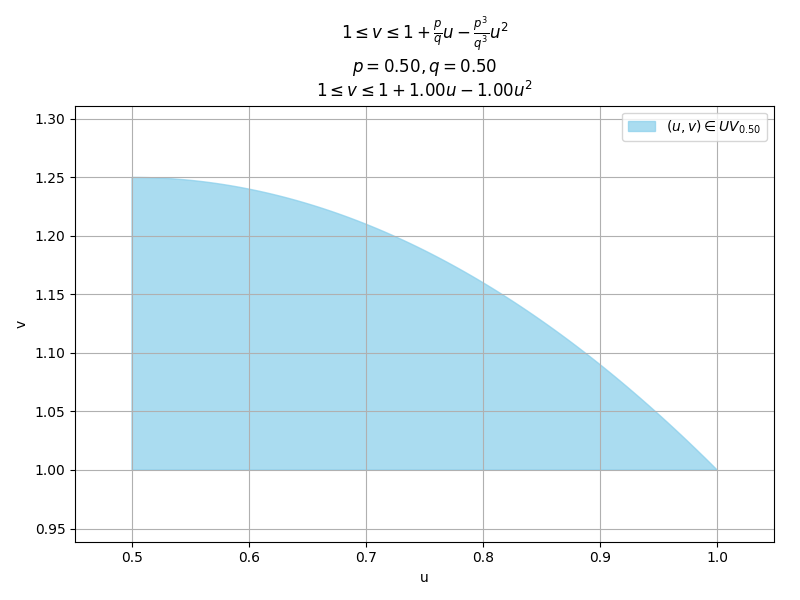
\includegraphics[width=0.48\linewidth]{figure/p=0.5}
%			\caption{The feasible region $UV_{0.5}$ for $p=0.5$}
%			\label{fig:p1}
%		\end{figure}
%		
%		\begin{figure}[!htbp]
%			\centering
%			\begin{subfigure}[b]{0.38\textwidth}
%				\centering
%				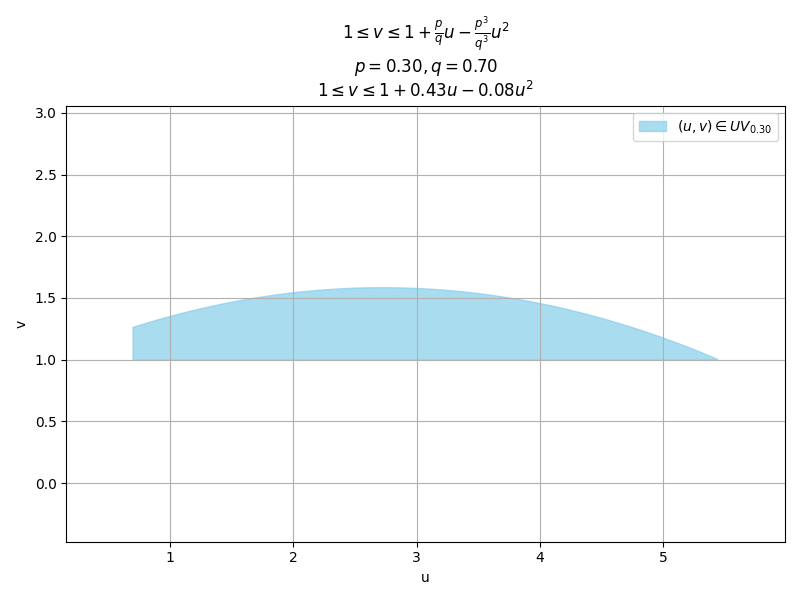
\includegraphics[width=\textwidth]{figure/p=0.3}
%				\caption{$p=0.3$}
%				\label{fig:p0}
%			\end{subfigure}
%			\hfill
%			\begin{subfigure}[b]{0.38\textwidth}
%				\centering
%				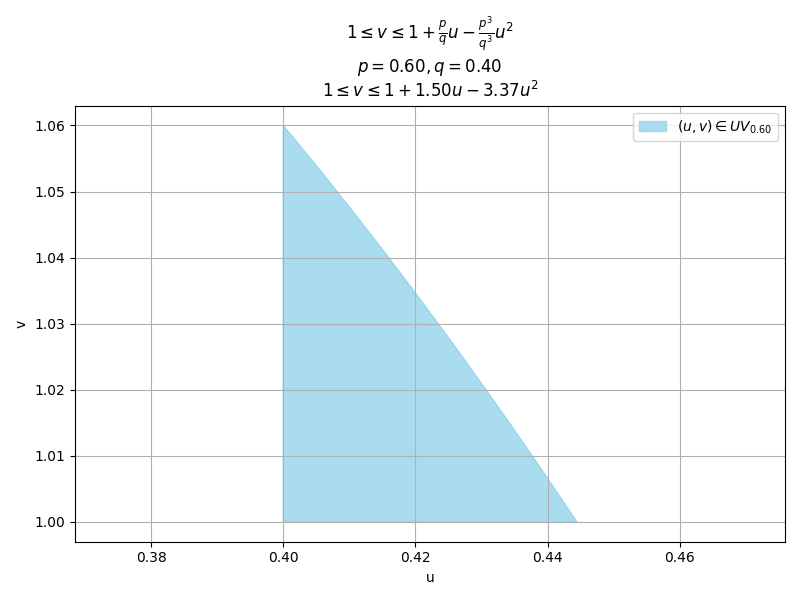
\includegraphics[width=\textwidth]{figure/p=0.6}
%				\caption{$p=0.6$}
%				\label{fig:p2}
%			\end{subfigure}
%			\caption{The feasible regions for $p=0.3$ and $p=0.6$}
%			\label{fig:combined}
%		\end{figure}
%		\end{example}
		
		\begin{figure}[!htbp]
			\centering
			\begin{subfigure}[b]{0.27\textwidth}
				\centering
				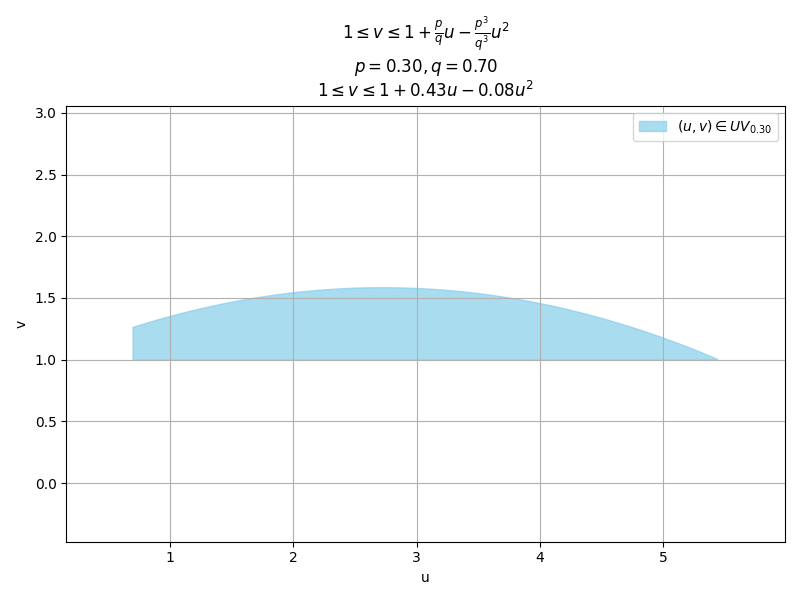
\includegraphics[width=\textwidth]{figure/p=0.3}
				\caption{$p=0.3$}
				\label{fig:p0}
			\end{subfigure}
			\hfill
			\begin{subfigure}[b]{0.27\textwidth}
				\centering
				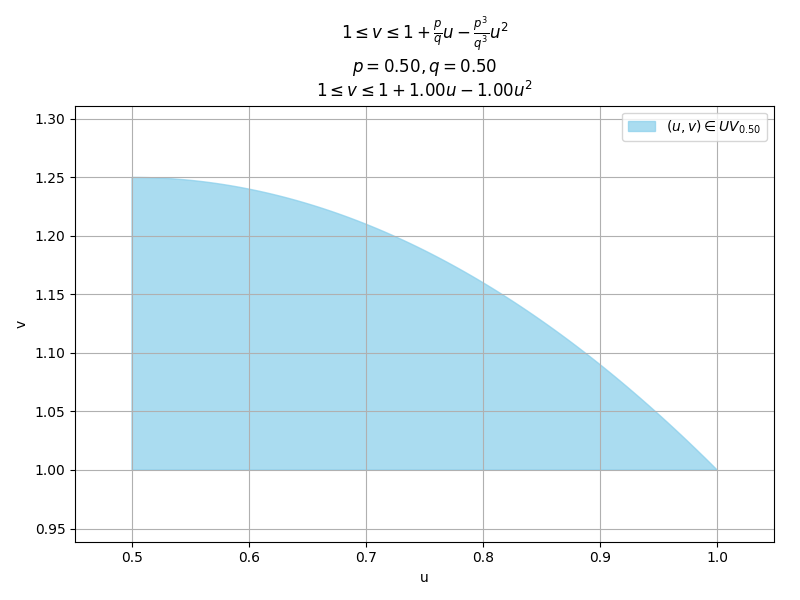
\includegraphics[width=\linewidth]{figure/p=0.5}
				\caption{$p=0.5$}
				\label{fig:p1}
			\end{subfigure}
			\hfill
			\begin{subfigure}[b]{0.27\textwidth}
				\centering
				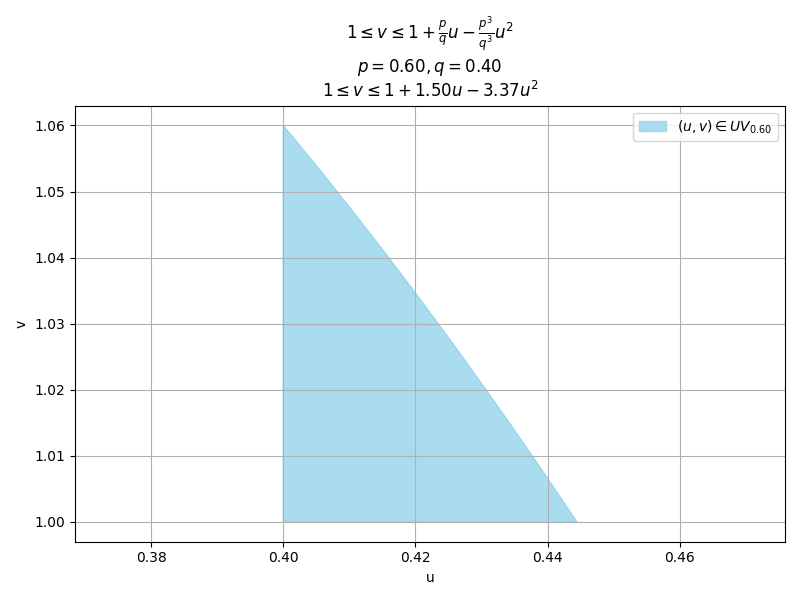
\includegraphics[width=\textwidth]{figure/p=0.6}
				\caption{$p=0.6$}
				\label{fig:p2}
			\end{subfigure}
			\caption{The feasible regions for $p=0.3$, $p=0.5$ and $p=0.6$}
			\label{fig:combined}
		\end{figure}
	\end{example}
	
	Let $s=(x_1,x_2,\cdots,x_l)$ be a segment of $x^*$ with $x_{l+1}=0$, $x_{-1}=x_{n-1}=Ux_1$, $x_0=x_n=0$. From the result of Theorem 3.14,
	\[
	\left( \frac{U^2}{q^2 x_l}, \frac{x_{l-1}}{p^2 x_l^2}, \frac{x_{l-2}}{(p x_{l-1} + q x_l)^2}, \cdots, \frac{x_2}{(p x_3 + q x_4)^2}, \frac{x_1}{(p x_2 + q x_3)^2} \right) = \mu (x_1, x_2, \cdots, x_l).
	\]
	\[
	\frac{1}{\mu}=\frac{q^2 x_1 x_l}{U^2}=\frac{p^2 x_2 x_l^2}{x_{l-1}}
	\]
	\[
	x_2 = \frac{q^2 x_1 x_{l-1}}{p^2 U^2 x_l}=\frac{q^2(V-1)}{p^2 U^2}x_1.
	\]
	For all $i=3,4,\ldots,l+2$, $x_{i-2}\neq 0$, we have $\partial_{i-2}F(x,p)=0$.
	\begin{equation*}
		\partial_{i-2}F(x,p) = \frac{1}{px_{i-1} + qx_i} - \frac{qx_{i-4}}{(px_{i-3} + qx_{i-2})^2} - \frac{px_{i-3}}{(px_{i-2} + qx_{i-1})^2} = 0
	\end{equation*}
	\begin{equation*}
		x_i = \frac{1}{\dfrac{q^2x_{i-4}}{(px_{i-3} + qx_{i-2})^2} + \dfrac{pqx_{i-3}}{(px_{i-2} + qx_{i-1})^2}} - \frac{p}{q} \cdot x_{i-1}.
	\end{equation*}
	Let $x_i=f_i^l x_1$ (the superscript $l$ is an index, not an exponent). Then $f_{-1}^l = U$, $f_0^l = 0$, $f_1^l = 1$, $f_2^l = \frac{q^2(V-1)}{p^2 U^2}$, and for $i\geq 3$,
	\begin{equation*}
		f_i^l = \frac{1}{\dfrac{q^2f_{i-4}^l}{(pf_{i-3}^l + qf_{i-2}^l)^2} + \dfrac{pqf_{i-3}^l}{(pf_{i-2}^l + qf_{i-1}^l)^2}} - \frac{p}{q}f_{i-1}^l.
	\end{equation*}
	
	\begin{example}
		Write a Python program \textup{\cite{wang2026}} using the SymPy package to compute $f_i^l$ for specified $i\geq -1$.
		\[
		f_3^l=\frac{p u - q v + q}{p u^{2}}.
		\]
		\[
		f_4^l=\frac{- p^{2} u + p q v - p q + q^{2}}{p q u^{2}}.
		\]
		\[
		f_5^l=\frac{p^{3} u v - p^{3} u + p^{2} q u - p^{2} q v^{2} + 2 p^{2} q v - p^{2} q - 2 p q^{2} v + 2 p q^{2}}{p q^{2} u^{2} v - p q^{2} u^{2} + q^{3} u^{2}}.
		\]
%		$
%		f_6^l=(- p^{7} u^{2} v^{3} + 3 p^{7} u^{2} v^{2} - 3 p^{7} u^{2} v + p^{7} u^{2} - 3 p^{6} q u^{2} v^{2} + 6 p^{6} q u^{2} v - 3 p^{6} q u^{2} + 2 p^{6} q u v^{4} - 8 p^{6} q u v^{3} + 12 p^{6} q u v^{2}
%		- 8 p^{6} q u v + 2 p^{6} q u - 3 p^{5} q^{2} u^{2} v + 3 p^{5} q^{2} u^{2} + 7 p^{5} q^{2} u v^{3} - 21 p^{5} q^{2} u v^{2} + 21 p^{5} q^{2} u v - 7 p^{5} q^{2} u - p^{5} q^{2} v^{5} + 5 p^{5} q^{2} v^{4}
%		- 10 p^{5} q^{2} v^{3} + 10 p^{5} q^{2} v^{2} - 5 p^{5} q^{2} v + p^{5} q^{2} - p^{4} q^{3} u^{2} + 7 p^{4} q^{3} u v^{2} - 14 p^{4} q^{3} u v + 7 p^{4} q^{3} u - 4 p^{4} q^{3} v^{4} + 16 p^{4} q^{3} v^{3}
%		- 24 p^{4} q^{3} v^{2} + 16 p^{4} q^{3} v - 4 p^{4} q^{3} + 2 p^{3} q^{4} u v - 2 p^{3} q^{4} u - 4 p^{3} q^{4} v^{3} + 12 p^{3} q^{4} v^{2} - 12 p^{3} q^{4} v + 4 p^{3} q^{4} + p q^{6} v - p q^{6} + q^{7})/(p^{4} q^{3} u^{3} v^{3} - 3 p^{4} q^{3} u^{3} v^{2} + 3 p^{4} q^{3} u^{3} v - p^{4} q^{3} u^{3} + 3 p^{3} q^{4} u^{3} v^{2} - 6 p^{3} q^{4} u^{3} v + 3 p^{3} q^{4} u^{3} - p^{3} q^{4} u^{2} v^{4} + 4 p^{3} q^{4} u^{2} v^{3} - 6 p^{3} q^{4} u^{2} v^{2} + 4 p^{3} q^{4} u^{2} v - p^{3} q^{4} u^{2} + 3 p^{2} q^{5} u^{3} v - 3 p^{2} q^{5} u^{3} - 3 p^{2} q^{5} u^{2} v^{3} + 9 p^{2} q^{5} u^{2} v^{2} - 9 p^{2} q^{5} u^{2} v + 3 p^{2} q^{5} u^{2} + p q^{6} u^{3} - 2 p q^{6} u^{2} v^{2} + 4 p q^{6} u^{2} v - 2 p q^{6} u^{2}).
%		$
		\\
		
		For $p=0.3$, compute $f_6^l=(- 0.0002187 u^{2} v^{3} - 0.0008748 u^{2} v^{2} - 0.0011664 u^{2} v - 0.0005184 u^{2} + 0.0010206 u v^{4} + 0.0042525 u v^{3} + 0.0005670 u v^{2} - 0.0050085 u v - 0.0008316 u - 0.0011907 v^{5} - 0.0051597 v^{4} + 0.0066150 v^{3} + 0.0230202 v^{2} - 0.0039984 v + 0.0630679)/(0.0027783 u^{3} v^{3} + 0.0111132 u^{3} v^{2} + 0.0148176 u^{3} v + 0.0065856 u^{3} - 0.0064827 u^{2} v^{4} - 0.0194481 u^{2} v^{3} + 0.0266511 u^{2} v^{2} + 0.0309729 u^{2} v - 0.0316932 u^{2})$.
	\end{example}
	
	That is, from $(U,V)$ and $x_1$, all elements of this segment $\{x_i\}_{i=1}^{l}$ can be determined. If $P(n,p)=\min\limits_{x \in K_n} F(x,p)=F(x^*,p)$ is attained at some $x^*\in K_n^{\bullet}$, and $x^*$ contains a segment of length $l$, then there must exist a point $(U,V)$ in the feasible region $UV_p$ determined by $p$ such that for all $i=1,2,\cdots,l$, $f_i^l>0$, and $f_{l+1}^l=0$.
	
	By Corollary 3.13, if $P(n,p)=\min\limits_{x \in K_n} F(x,p)=F(x^*,p)$ is attained at some $x^*\in K_n^{\bullet}$, then any two segments $s$ and $t$ of $x^*$ having the same length $l$ must be proportional, thus share the same value of $V$. For $x\in K_n^{\bullet}$, we define $R_l(x^*)=\frac{\Head(s)}{\Tail(s)}$. From the above derivation, $R_l(x^*)=\frac{1}{f_l^l}$. For a segment of length $1$, $R_1(x^*)=1$. Note the definitions of $U$ and $R$. For $x=(s_1,0,s_2,0,\cdots,s_k,0)$ with pattern $(l_1,l_2,\cdots,l_k)$, we have the relation
	\[
	U(x)^k R_{l_1}R_{l_2}\cdots R_{l_k}=1.
	\]
	
	In $UV_p$, consider the set of points $(u,v)$ such that for all $i=1,2,\cdots,l$, $f_i^l(u,v)>0$ and $f_{l+1}^l(u,v)=0$. Then the projection of this set onto $U$ yields an interval, and $R_l(x^*)=\frac{1}{f_l^l}$ also ranges over some interval on this set.
	
	For given $n$ and $p$, consider all possible patterns $(l_1,l_2,\cdots,l_k)$ with total length $n$. Compute the feasible region $UV_p$ and ranges of $U$ and $R_l$ in $UV_p$ corresponding to each $l_i$. If the minimizer has pattern $(l_1,l_2,\cdots,l_k)$, then the $U$ ranges must have a nonempty intersection, and the equation $U^k R_{l_1}R_{l_2}\cdots R_{l_k}=1$ must have a solution within that intersection. That is, we need to solve the following problem:
	
	Find $(u,v_1,v_2,\cdots,v_k)$ satisfying:
	\[
	\left\{
	\begin{array}{l}
		\forall i=1,2,\ldots,k, \\
		\qquad (u,v_i)\in UV_p=\left\{(u,v)\mid q\leq u\leq\frac{q^2}{p^2},1\leq v\leq1+\frac{p}{q}u-\frac{p^3}{q^3}u^2\right\}\\
		\qquad \forall j=1,2,\ldots,l_i, \quad f_j^{l_i}(u, v_i) > 0, \quad f_{l_i+1}^{l_i}(u, v_i) = 0. \\
		u^k = f_{l_1}^{l_1}(u, v_1) \cdot f_{l_2}^{l_2}(u, v_2) \cdots f_{l_k}^{l_k}(u, v_k).
	\end{array}
	\right.\tag{Q}
	\]
	
	In fact, for all $j \geq -1$, the expressions $f_j^{l_i}$ are the same rational functions in $(u,v)$ regardless of $l_i$; we may omit the superscript. The closure conditions in the above problem can be reduced to a system of polynomial equations.
	
	By Corollary 3.13 and Theorem 3.6(2), we can group segments of the same length together. Suppose the minimizer has pattern
	\[
	(\underbrace{l_1,\cdots,l_1}_{m_1\text{ times}},\underbrace{l_2,\cdots,l_2}_{m_2\text{ times}},\cdots,\underbrace{l_k,\cdots,l_k}_{m_k\text{ times}}).
	\]
	The above problem can be reformulated as follows.
	
	Find $(u, v_1, \cdots, v_k)$ satisfying:
	\[
	\left\{
	\begin{array}{l}
		f_{l_i+1}(u, v_i) = 0 \quad \quad i=1,2,\cdots,k \qquad \qquad\text{(i)}\\
		u^{m_1+\cdots+m_k} = (f_{l_1}(u,v_1))^{m_1} \cdot (f_{l_2}(u,v_2))^{m_2} \cdots (f_{l_k}(u,v_k))^{m_k} \qquad\qquad \text{(k+1)}\\
		q\leq u\leq\frac{q^2}{p^2}\\
		\forall~i=1,2,\ldots,k, \quad 1 \leq v_i \leq 1 + \dfrac{p}{q}u - \dfrac{p^3}{q^3}u^2\\
		\qquad\forall~j=1,2,\ldots,l_i, \quad f_j(u,v_i) > 0.
	\end{array}
	\right.
	\tag{Q}
	\]
	
	In fact, this problem often has no solution. Since the total number of possible patterns for a given total length $n$ is finite, we can check them one by one and identify all patterns that admit a solution. If no pattern yields a solution, then $P(n,p)=\min\limits_{x \in K_n}F(x,p)=\min\limits_{x \in K_n^{\circ}}F(x,p)$, which is the trivial case, and the result follows from Theorem 3.12(2).
	
	If there are several patterns with solutions, note that for each pattern, the solution set lies in the compact set
	\[
	(u,v_1,v_2,\cdots,v_k)\in \left[q,\frac{q^2}{p^2}\right]\times {\left[1,1+\frac{q^4}{4p^4}\right]}^k =\widetilde{UV_p}\subset \mathbb{R}^{k+1}.
	\]
	Then by Definition 3.8,
	\begin{align*}
		\widetilde{F(u,v)}=F(x,p) &= \frac{r}{q} U(x) + \sum_{i=1}^k \Sop(s_i) \\
		&= \frac{r}{q} u + \sum_{i=1}^k \sum_{j=1}^{l_i - 1} \frac{x_j}{p x_{j+1} + q x_{j+2}} \text{ (the } j\text{-th element of the } i\text{-th segment)} \\
		&= \frac{r}{q} u + \sum_{i=1}^k \sum_{j=1}^{l_i - 1} \frac{f_j(u,v_i)}{p f_{j+1}(u,v_i) + q f_{j+2}(u,v_i)}
	\end{align*}
	is a continuous function on this compact set and therefore attains a minimum. In fact, for patterns with solutions, the solution set often consists of only a few isolated points. We can compute these minima, compare the minimal values among the finitely many patterns that admit solutions, and then compare with the trivial case value $n$ in Theorem 3.12(2) to obtain $P(n,p)=\min\limits_{x \in K_n}F(x,p)$.
	
	\subsubsection{Procedure for Finding the Minimum of the Denominator-Weighted Shapiro Cyclic Sum}
	
	\begin{enumerate}
		\item For a given positive integer $n\geq 3$ and $0<p<1$, list all finitely many possible patterns $(l_1,l_2,\cdots,l_k)$ satisfying $l_1\geq l_2\geq\cdots\geq l_k$ and $l_1+ l_2+\cdots+ l_k +k=n$.
		\item For each pattern, perform the following:
		\begin{enumerate}
			\item Combine segments of the same length and rewrite the pattern in the form:
			\[
			(\underbrace{l_1,\cdots,l_1}_{m_1\text{ times}},\underbrace{l_2,\cdots,l_2}_{m_2\text{ times}},\cdots,\underbrace{l_k,\cdots,l_k}_{m_k\text{ times}}).
			\]
			\item Solve the system of equations in $(u, v_1, \cdots, v_k)$:
			\[
			\left\{
			\begin{array}{l}
				f_{l_i+1}(u, v_i) = 0 \quad \quad i=1,2,\cdots,k \qquad \qquad\text{(i)}\\
				u^{\sum_{i=1}^{k}m_i} = \prod_{i=1}^{k}(f_{l_i}(u,v_i))^{m_i} \qquad\qquad \text{(k+1)}\\
				q\leq u\leq\frac{q^2}{p^2}\\
				\forall~i=1,2,\ldots,k, \quad 1 \leq v_i \leq 1 + \dfrac{p}{q}u - \dfrac{p^3}{q^3}u^2\\
				\qquad\forall~j=1,2,\ldots,l_i, \quad f_j(u,v_i) > 0.
			\end{array}
			\right.
			\tag{Q}
			\]
			\item If the system has no solution, discard this pattern. If the system has a solution, substitute to obtain the value of $\widetilde{F(u,v)}= \frac{r}{q} u + \sum_{i=1}^k m_i \sum_{j=1}^{l_i - 1} \frac{f_j(u,v_i)}{p f_{j+1}(u,v_i) + q f_{j+2}(u,v_i)}$.
		\end{enumerate}
		\item Compare all finitely many $\widetilde{F(u,v)}$ obtained from solvable patterns with the trivial case value $n$ to obtain $P(n,p)=\min\limits_{x \in K_n}F(x,p)$.
	\end{enumerate}
	
	\begin{example}
		Find $P(6,0.3)$.
	\end{example}
	
	Consider all patterns with total length $6$: $(5)$, $(3,1)$, $(2,2)$, $(1,1,1)$.
	
	For pattern $(5)$, $(3,1)$ and $(2,2)$, the solutions of corresponding problems lie outside the feasible region. For example pattern (2,2), problem (Q) is to find $(u, v)$ satisfying:
	\[
	\left\{
	\begin{array}{l}
		f_{3}(u, v) = 0 \qquad \qquad\text{(1)}\\
		u= f_{2}(u,v) \qquad\qquad \text{(2)}\\
		0.7\leq u\leq \frac{49}{9}\\
		1 \leq v \leq 1 + \dfrac{3}{7}u - \dfrac{27}{343}u^2\\
		f_1(u,v),f_2(u,v)> 0.
	\end{array}
	\right.
	\tag{Q}
	\]
	Solving the system yields $(u,v)\approx(1.53,1.65)$, which lies outside the feasible region, so no solution.
	
%	For pattern $(5)$, problem (Q) is to find $(u, v)$ satisfying:
%	\[
%	\left\{
%	\begin{array}{l}
%		f_{6}(u, v) = 0 \qquad \qquad\text{(1)}\\
%		u= f_{5}(u,v) \qquad\qquad \text{(2)}\\
%		0.7\leq u\leq \frac{49}{9}\\
%		1 \leq v \leq 1 + \dfrac{3}{7}u - \dfrac{27}{343}u^2\\
%		\forall j=1,2,\ldots,5, \quad f_j(u,v) > 0.
%	\end{array}
%	\right.
%	\tag{Q}
%	\]
%	Solving the system yields $5$ solutions:
%	\begin{enumerate}
%		\item $(u, v) = (-1.000000000000000, 2.139260689980808)$
%		\item $(u, v) = (0.856124222290431, -4.278918663389620)$
%		\item $(u, v) = (855836625.917668700218201, -1.333333333333333)$
%		\item $(u, v) = (-855836631.822430610656738, -1.333333333333333)$
%		\item $(u, v) = (-1.000000000000000, -2.901165451885570)$
%	\end{enumerate}
%	None lie in the feasible region, so no solution.
%	
%	For pattern $(3,1)$, problem (Q) is to find $(u, v_1, v_2)$ satisfying:
%	\[
%	\left\{
%	\begin{array}{l}
%		f_{4}(u, v_1) = 0 \qquad \qquad\text{(1)}\\
%		f_{2}(u, v_2) = 0 \qquad \qquad\text{(2)}\\
%		u^{2} = f_{3}(u,v_1) \cdot f_{1}(u,v_2)  \qquad\qquad \text{(3)}\\
%		0.7\leq u\leq \frac{49}{9}\\
%		1 \leq v_1,v_2 \leq 1 + \dfrac{3}{7}u - \dfrac{27}{343}u^2\\
%		f_1(u,v_1),f_2(u,v_1),f_3(u,v_1),f_1(u,v_2) > 0.
%	\end{array}
%	\right.
%	\tag{Q}
%	\]
%	Solving the system yields $(u,v_1,v_2)=(\frac{\sqrt{21}}{3},\frac{3\sqrt{21}-28}{21},1)$, which lies outside the feasible region, so no solution.
%	
%	For pattern $(2,2)$, problem (Q) is to find $(u, v)$ satisfying:
%	\[
%	\left\{
%	\begin{array}{l}
%		f_{3}(u, v) = 0 \qquad \qquad\text{(1)}\\
%		u= f_{2}(u,v) \qquad\qquad \text{(2)}\\
%		0.7\leq u\leq \frac{49}{9}\\
%		1 \leq v \leq 1 + \dfrac{3}{7}u - \dfrac{27}{343}u^2\\
%		f_1(u,v),f_2(u,v)> 0.
%	\end{array}
%	\right.
%	\tag{Q}
%	\]
%	Solving the system yields $(u,v)\approx(1.53,1.65)$, which lies outside the feasible region, so no solution.
	
	For pattern $(1,1,1)$, by the AM-GM inequality, it is easy to see that the minimizer is of the form $(a,0,a,0,a,0)$, and the minimum value is $\frac{30}{7}$. Since $\frac{30}{7}<6$, it is smaller than the trivial case.
	
	In summary, $P(6,0.3)=\frac{30}{7}$.
	
	The above summarizes the general method for deriving the minimum of the denominator-weighted Shapiro cyclic sum. However, it is evident that the classification and computational effort are substantial. This method can strictly determine the minimum and minimizer of the Shapiro cyclic sum for small $n$; for large $n$, the main computational challenges are: (1) classification of patterns for $n$, (2) computation of the rational functions $f_i(u,v)$, and (3) solving systems of polynomial equations, all of which are quite difficult. In the following, we propose an efficient algorithm for solving the minimum of the denominator-weighted Shapiro cyclic sum.
	
	\section{Efficient RBFGS Algorithm for the Minimum of the Denominator-Weighted Shapiro Cyclic Sum}
	\subsection{Problem Transformation}
	
	The BFGS algorithm is an efficient method for solving unconstrained optimization problems. For the denominator-weighted Shapiro cyclic sum problem, let $x_i = y_i^2$. Then $y_i \in \mathbb{R}$ automatically ensures $x_i \geq 0$, transforming the problem into an unconstrained optimization problem in $y_i$. Implementing the BFGS algorithm for this problem reveals that either the range of feasible initial points is extremely narrow, making it difficult to find counterexamples or to exhibit global properties, or that when the initial point range is slightly expanded, the algorithm quickly diverges to the maximum or minimum representable by computer floating-point arithmetic, yielding poor performance.
	
	Furthermore, since the objective function is homogeneous of degree zero, we can add a normalization condition $\sum_{i=1}^n y_i^2 = 1$, i.e.,
	\[
	\min_{\mathbf{y} \in \mathbb{S}^{n-1}} f(\mathbf{y}) = \sum_{i=1}^{n} \frac{y_i^2}{p y_{i+1}^2 + q y_{i+2}^2},
	\]
	where $\mathbb{S}^{n-1} = \{\mathbf{y} \in \mathbb{R}^n \mid \|\mathbf{y}\|_2 = 1\}$ is the unit sphere, a compact Riemannian manifold.
	
%	\begin{definition}
%		The unit sphere $\mathbb{S}^{n-1}$ is a Riemannian manifold embedded in $\mathbb{R}^n$ with the following geometric structure:
%		
%		\begin{itemize}
%			\item \textbf{Tangent space}: The tangent space at a point $\mathbf{y} \in \mathbb{S}^{n-1}$ is
%			\[
%			T_{\mathbf{y}} \mathbb{S}^{n-1} = \{\mathbf{v} \in \mathbb{R}^n \mid \mathbf{y}^T \mathbf{v} = 0\}.
%			\]
%			\item \textbf{Projection map}: The projection mapping a Euclidean vector onto the tangent space is
%			\[
%			P_{\mathbf{y}}(\mathbf{v}) = \mathbf{v} - (\mathbf{y}^T \mathbf{v})\mathbf{y}.
%			\]
%			\item \textbf{Riemannian gradient}: The Euclidean gradient of the objective function is $\nabla f(\mathbf{y})$, and its Riemannian gradient is the projection:
%			\[
%			\text{grad} f(\mathbf{y}) = P_{\mathbf{y}}(\nabla f(\mathbf{y})).
%			\]
%		\end{itemize}
%	\end{definition}
%	
%	To implement the BFGS algorithm on the manifold, the following concepts are needed:
%	
%	\begin{definition}
%		A retraction $R_{\mathbf{y}}: T_{\mathbf{y}} \mathbb{S}^{n-1} \to \mathbb{S}^{n-1}$ maps a tangent vector back to the manifold, satisfying:
%		\begin{enumerate}
%			\item $R_{\mathbf{y}}(\mathbf{0}) = \mathbf{y}$,
%			\item $\frac{d}{dt} R_{\mathbf{y}}(t\boldsymbol{\eta})|_{t=0} = \boldsymbol{\eta}$.
%		\end{enumerate}
%		For the unit sphere, the normalization retraction is used:
%		\[
%		R_{\mathbf{y}}(\boldsymbol{\eta}) = \frac{\mathbf{y} + \boldsymbol{\eta}}{\|\mathbf{y} + \boldsymbol{\eta}\|}.
%		\]
%	\end{definition}
	
	\begin{definition}[\cite{qi2011}]
		A vector transport $\mathcal{T}_{\mathbf{y} \to \mathbf{z}}: T_{\mathbf{y}} \mathbb{S}^{n-1} \to T_{\mathbf{z}} \mathbb{S}^{n-1}$ maps tangent vectors between different tangent spaces, requiring linearity and preservation of inner products. Common approaches include projection transport and parallel transport. This paper adopts parallel transport:
		\[
		\mathcal{T}_{\boldsymbol{\eta}}(\boldsymbol{\xi}) =\mathcal{T}_{\mathbf{y} \to \mathbf{z}}= \boldsymbol{\xi} - \frac{(\mathbf{y} + \mathbf{z})^T \boldsymbol{\xi}}{1 + \mathbf{y}^T \mathbf{z}} (\mathbf{y} + \mathbf{z}),
		\]
		where $\mathbf{z} = R_{\mathbf{y}}(\boldsymbol{\eta})$.
	\end{definition}
	
	\subsection[Riemannian BFGS (RBFGS) Algorithm Procedure]
	{Riemannian BFGS (RBFGS) Algorithm Procedure\hfill\small\textmd{(summarized from \cite{ring2012}\cite{huang2015})}}
	
	\begin{enumerate}
		\item Initialization: Choose $\mathbf{y}_0 \in \mathbb{S}^{n-1}$, set $H_0 = I_{n}$.
		\item For $k = 0,1,2,\ldots$, do:
		\begin{enumerate}
			\item Compute the Riemannian gradient $\mathbf{g}_k = \text{grad} f(\mathbf{y}_k)$. If the norm of the Riemannian gradient is less than a preset tolerance or the maximum number of iterations is exceeded, output $\mathbf{y}_k$ and terminate.
			\item Compute the search direction $\boldsymbol{\eta}_k = -H_k \mathbf{g}_k$.
			\item Determine the step size $\alpha_k$ via a Wolfe line search.
			\item Update the point: $\mathbf{y}_{k+1} = R_{\mathbf{y}_k}(\alpha_k \boldsymbol{\eta}_k)$.
			\item Compute the transported vectors:
			\[
			\mathbf{s}_k = \mathcal{T}_{\alpha_k \boldsymbol{\eta}_k}(\alpha_k \boldsymbol{\eta}_k), \quad
			\mathbf{y}_k^{\text{grad}} = \text{grad} f(\mathbf{y}_{k+1}) - \mathcal{T}_{\alpha_k \boldsymbol{\eta}_k}(\text{grad} f(\mathbf{y}_k)).
			\]
			\item Update the inverse Hessian approximation using the BFGS formula:
			\[
			H_{k+1} = \left(I - \frac{\mathbf{s}_k (\mathbf{y}_k^{\text{grad}})^T}{\langle \mathbf{s}_k, \mathbf{y}_k^{\text{grad}} \rangle} \right) H_k \left(I - \frac{\mathbf{y}_k^{\text{grad}} \mathbf{s}_k^T}{\langle \mathbf{s}_k, \mathbf{y}_k^{\text{grad}} \rangle} \right) + \frac{\mathbf{s}_k \mathbf{s}_k^T}{\langle \mathbf{s}_k, \mathbf{y}_k^{\text{grad}} \rangle}.
			\]
		\end{enumerate}
	\end{enumerate}
	
	\subsection{Numerical Experiments and Algorithm Enhancements}
	
	\textbf{Oscillatory Solution Detection and Restart Mechanism}
	
	Numerical experiments reveal that for even $n$, the solution often converges to an oscillatory form $(a,b,a,b,\ldots)$, at which the gradient is zero. Referring to Theorem 3.12, this is likely merely a local stationary point. Moreover, several important counterexamples to the classical Shapiro inequality are near this $(a,b,a,b,\ldots)$ pattern. Therefore, a detection mechanism is added:
	\[
	\text{is\_alternating}(\mathbf{y}) = 
	\begin{cases}
		\text{True}, & \text{std}(y_{\text{odd}}) < \epsilon \text{ and std}(y_{\text{even}}) < \epsilon \\
		\text{False}, & \text{otherwise}
	\end{cases}
	\]
	
	When an oscillatory solution is detected with $f(\mathbf{y}) \geq n$, a random perturbation is applied to the current solution:
	\[
	\mathbf{y}_{\text{perturbed}} = \frac{\mathbf{y} + \delta \mathbf{r}}{\|\mathbf{y} + \delta \mathbf{r}\|}, \quad \mathbf{r} \sim \mathcal{N}(0,I_n),
	\]
	and the optimization is restarted from the perturbed point, repeated at most 10 times (or a specified number).
	
	\textbf{Maintaining the Curvature Condition}
	
	In Euclidean space, %From the derivation in Lemma 2.4, in Euclidean space, 
	if the initial $H_0$ is positive definite and the step size satisfies the curvature condition
	\[
	\nabla f(x^{(k)} + \lambda d^{(k)})^{T} d^{(k)} \geq c_2 \, \nabla f(x^{(k)})^{T} d^{(k)},
	\]
	then the curvature condition and the positive definiteness of $H_k$ hold for all iterations.
	
	On the unit sphere, it often occurs that after several iterations the curvature condition is no longer satisfied. If the iteration continues, the positive definiteness of $H_k$ cannot be maintained, and the function value increases significantly, deviating from the objective. Therefore, a curvature monitoring mechanism is added: if no step size satisfying the Wolfe line search conditions is found, the step size is determined via an Armijo line search, and $H_k$ is reset to $I_n$.
	
	Additionally, the algorithm incorporates other measures to ensure safe computation: (1) safe norm and safe division to avoid numerical overflow, and (2) gradient clipping to control update magnitudes.
	
	\textbf{Convergence Analysis}
	
	Based on the above content, write a Python program \cite{wang2026} to conduct numerical experiments. The algorithm exhibits good convergence across problems of various scales:
	
	\begin{itemize}
		\item The gradient norm converges to zero.
		\item The objective function value of Shapiro cyclic sum converges stably within each run.
		\item For the four sets of critical values of the classical Shapiro inequality, namely $p=0.5$, $n = 12, 14$ and $n = 23, 25$, the algorithm performs well, finding counterexamples for $n=14, 25$ within 10 perturbations.
	\end{itemize}
	
%	\begin{figure}[!htbp]
%		\centering
%		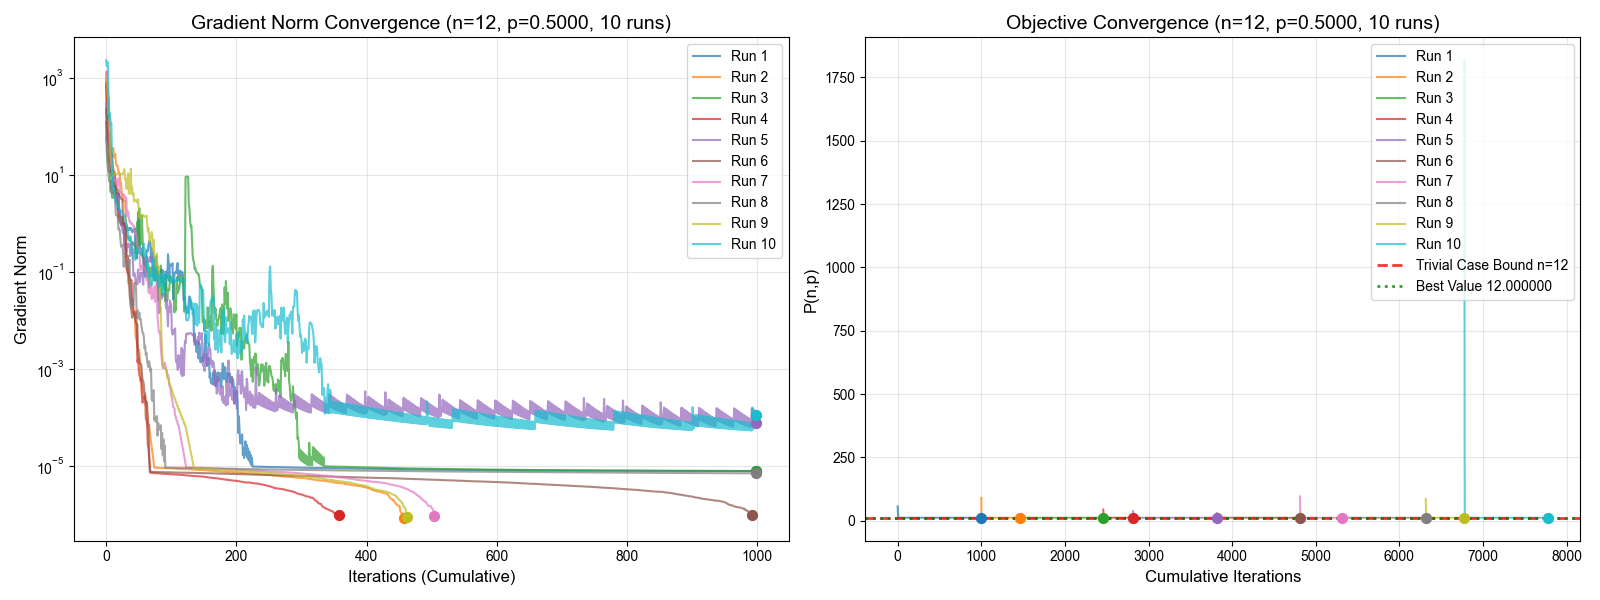
\includegraphics[width=0.7\linewidth]{figure/n=12,p=0.5}
%		\caption{Convergence of Shapiro Cyclic Sum and Gradient Norm ($n=12, p=0.5$)}
%		\label{fig:n12p05}
%	\end{figure}
%	\begin{figure}[!htbp]
%		\centering
%		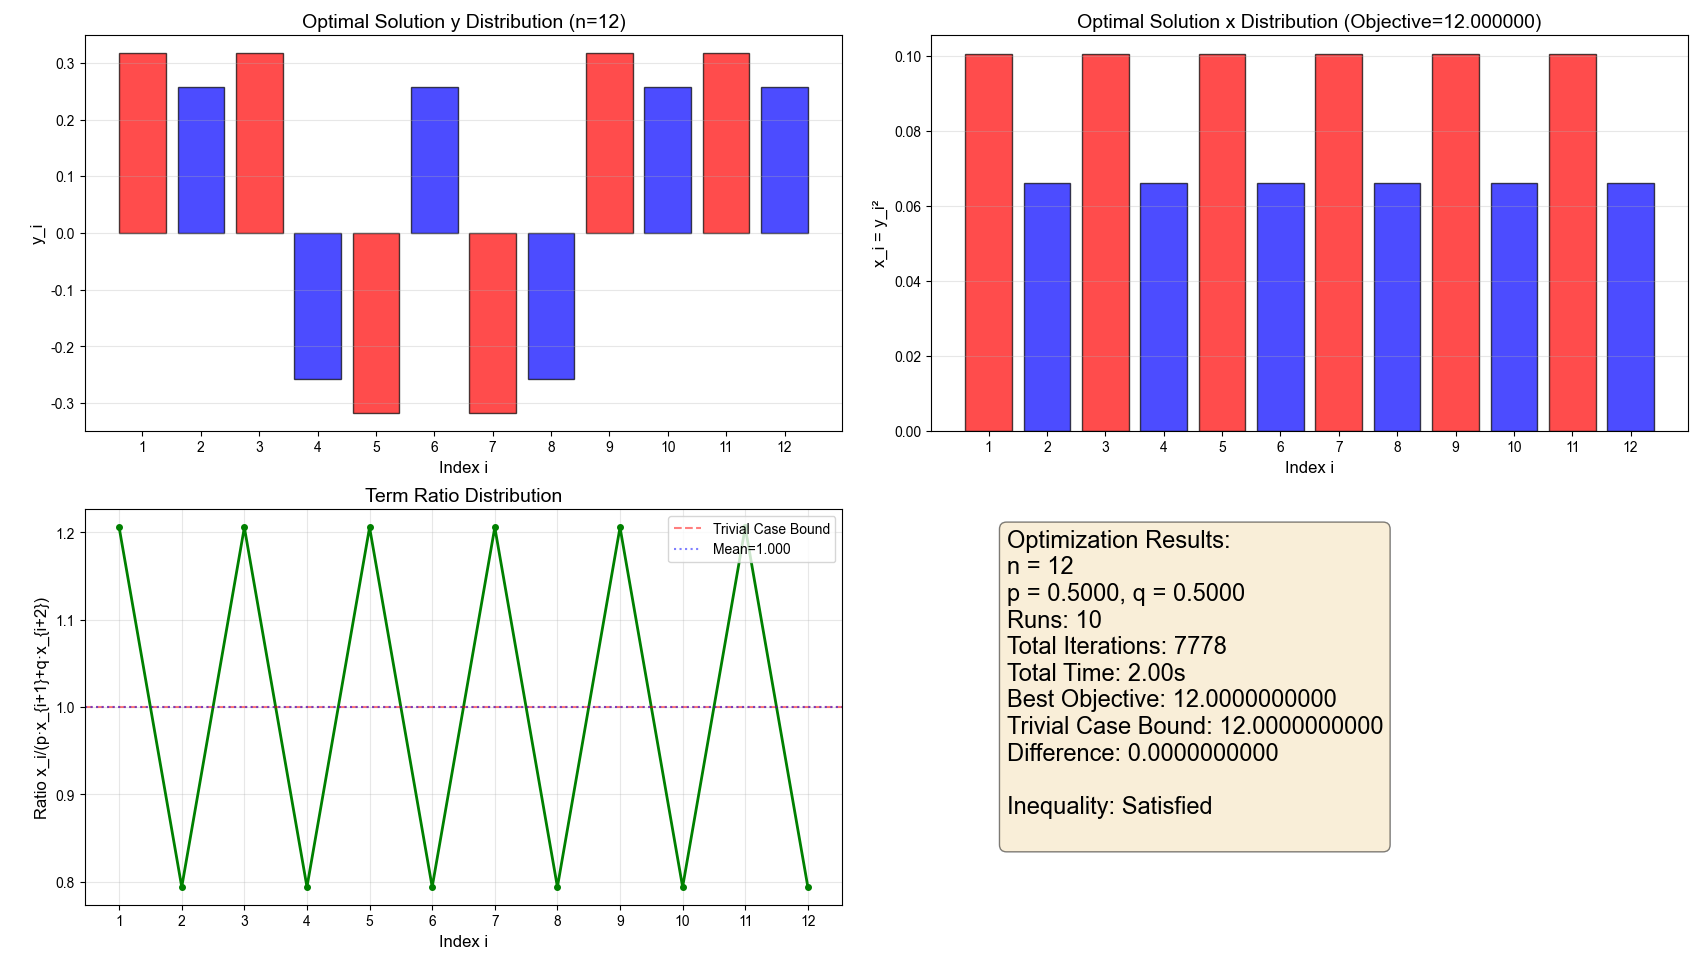
\includegraphics[width=0.55\linewidth]{figure/n=12,p=0.5_1}
%		\caption{Optimal Solution Distribution ($n=12, p=0.5$)}
%		\label{fig:n12p05_1}
%	\end{figure}
	
	\begin{figure}[!htbp]
		\centering
		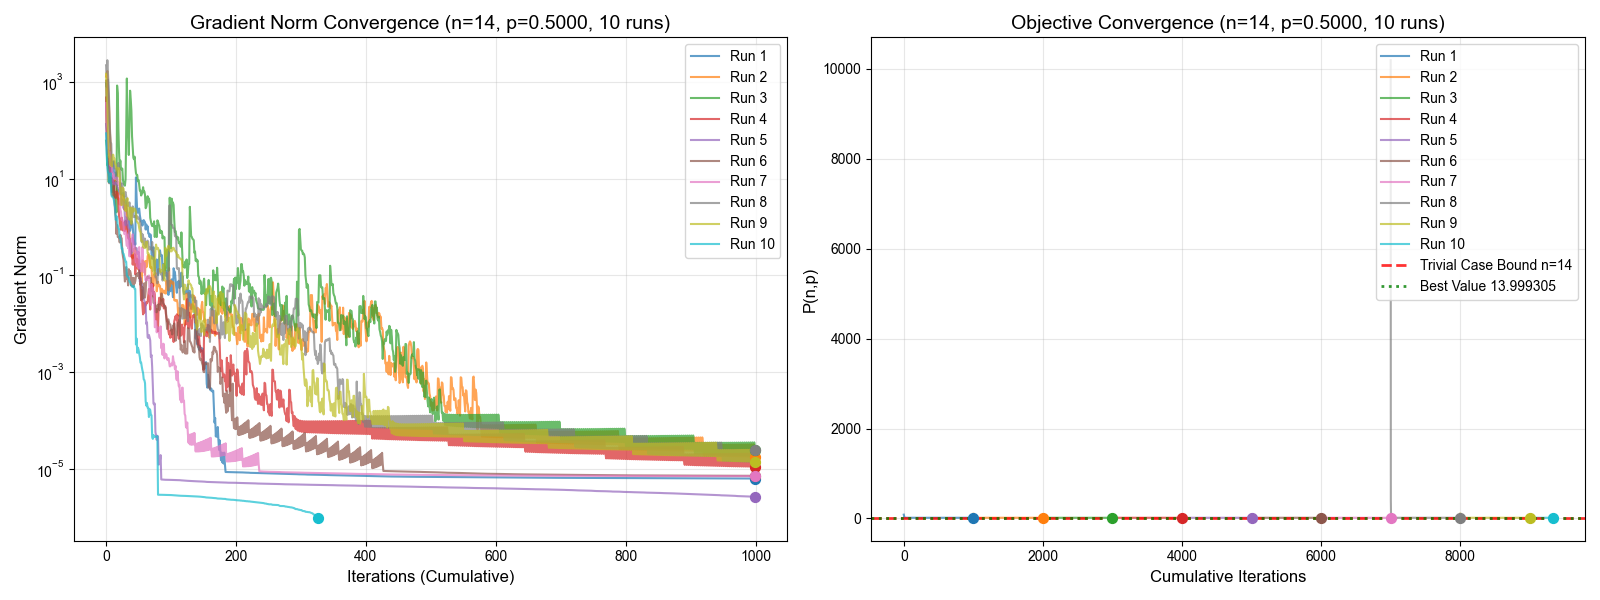
\includegraphics[width=0.55\linewidth]{figure/n=14,p=0.5}
		\caption{Convergence of Shapiro Cyclic Sum and Gradient Norm ($n=14, p=0.5$)}
		\label{fig:n14p05}
	\end{figure}
	\begin{figure}[!htbp]
		\centering
		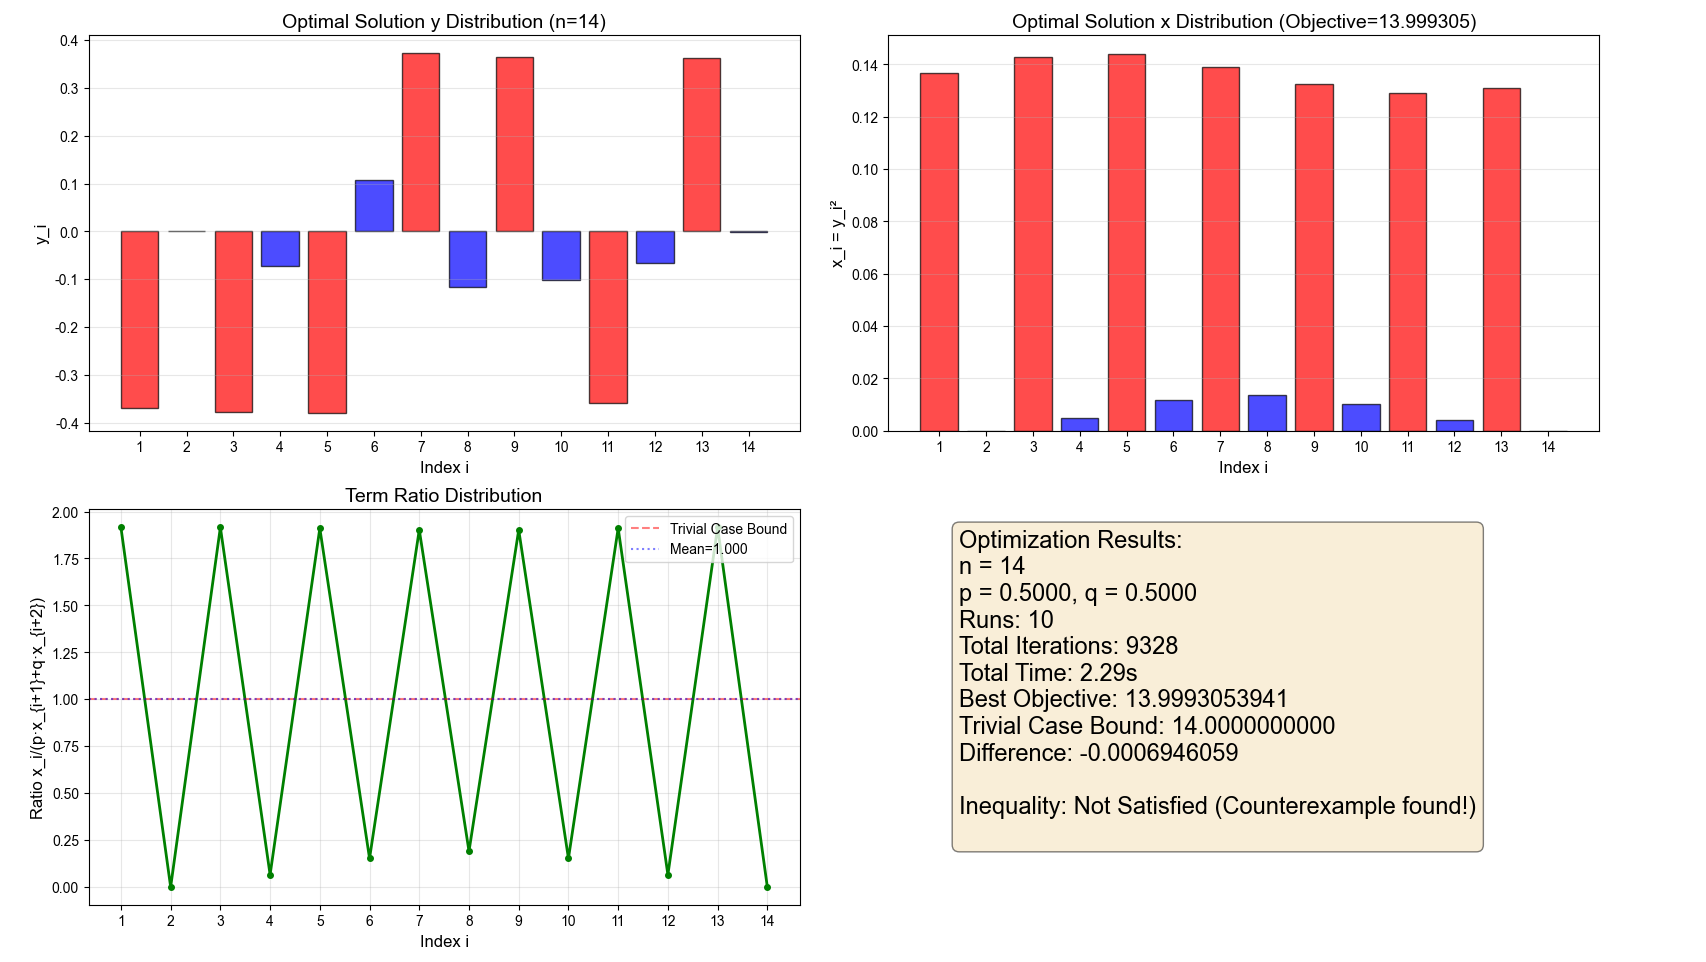
\includegraphics[width=0.55\linewidth]{figure/n=14,p=0.5_1}
		\caption{Optimal Solution Distribution ($n=14, p=0.5$)}
		\label{fig:n14p05_1}
	\end{figure}
	
%	\begin{figure}[!htbp]
%		\centering
%		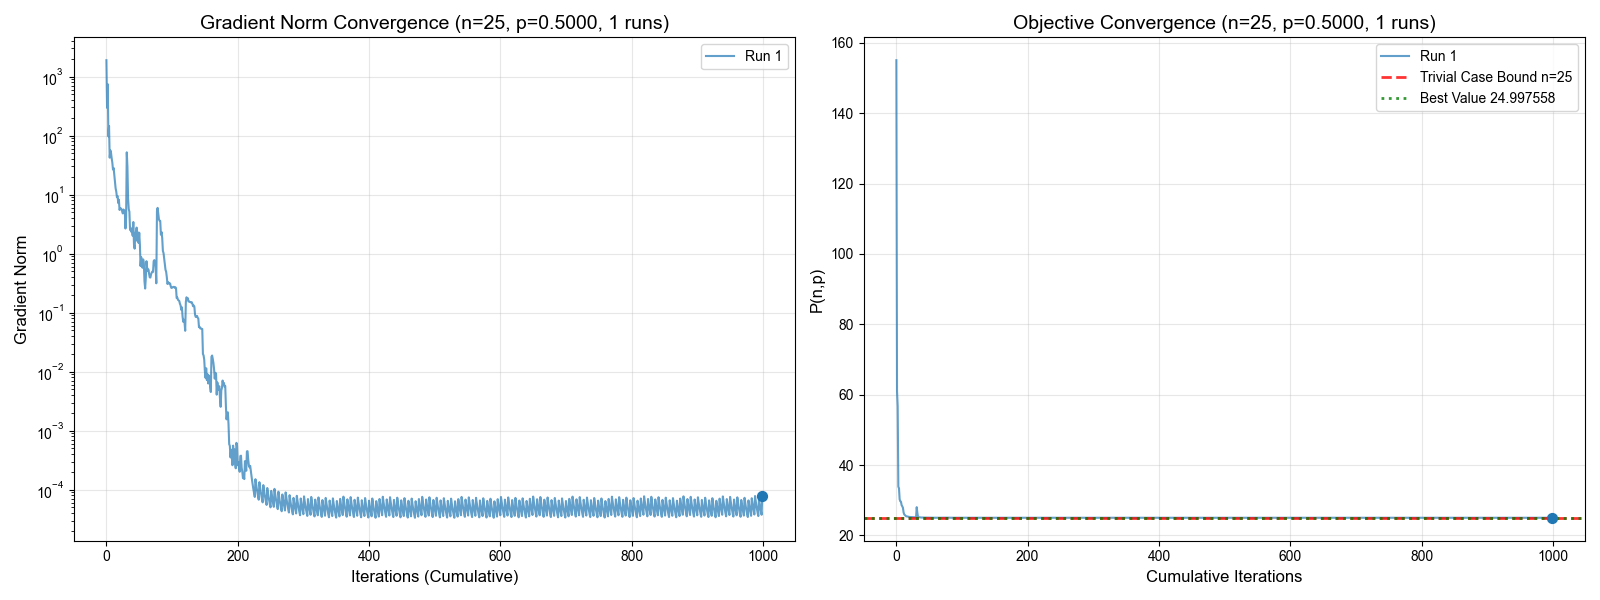
\includegraphics[width=0.55\linewidth]{figure/n=25,p=0.5}
%		\caption{Convergence of Shapiro Cyclic Sum and Gradient Norm ($n=25, p=0.5$)}
%		\label{fig:n25p05}
%	\end{figure}
%	\begin{figure}[!htbp]
%		\centering
%		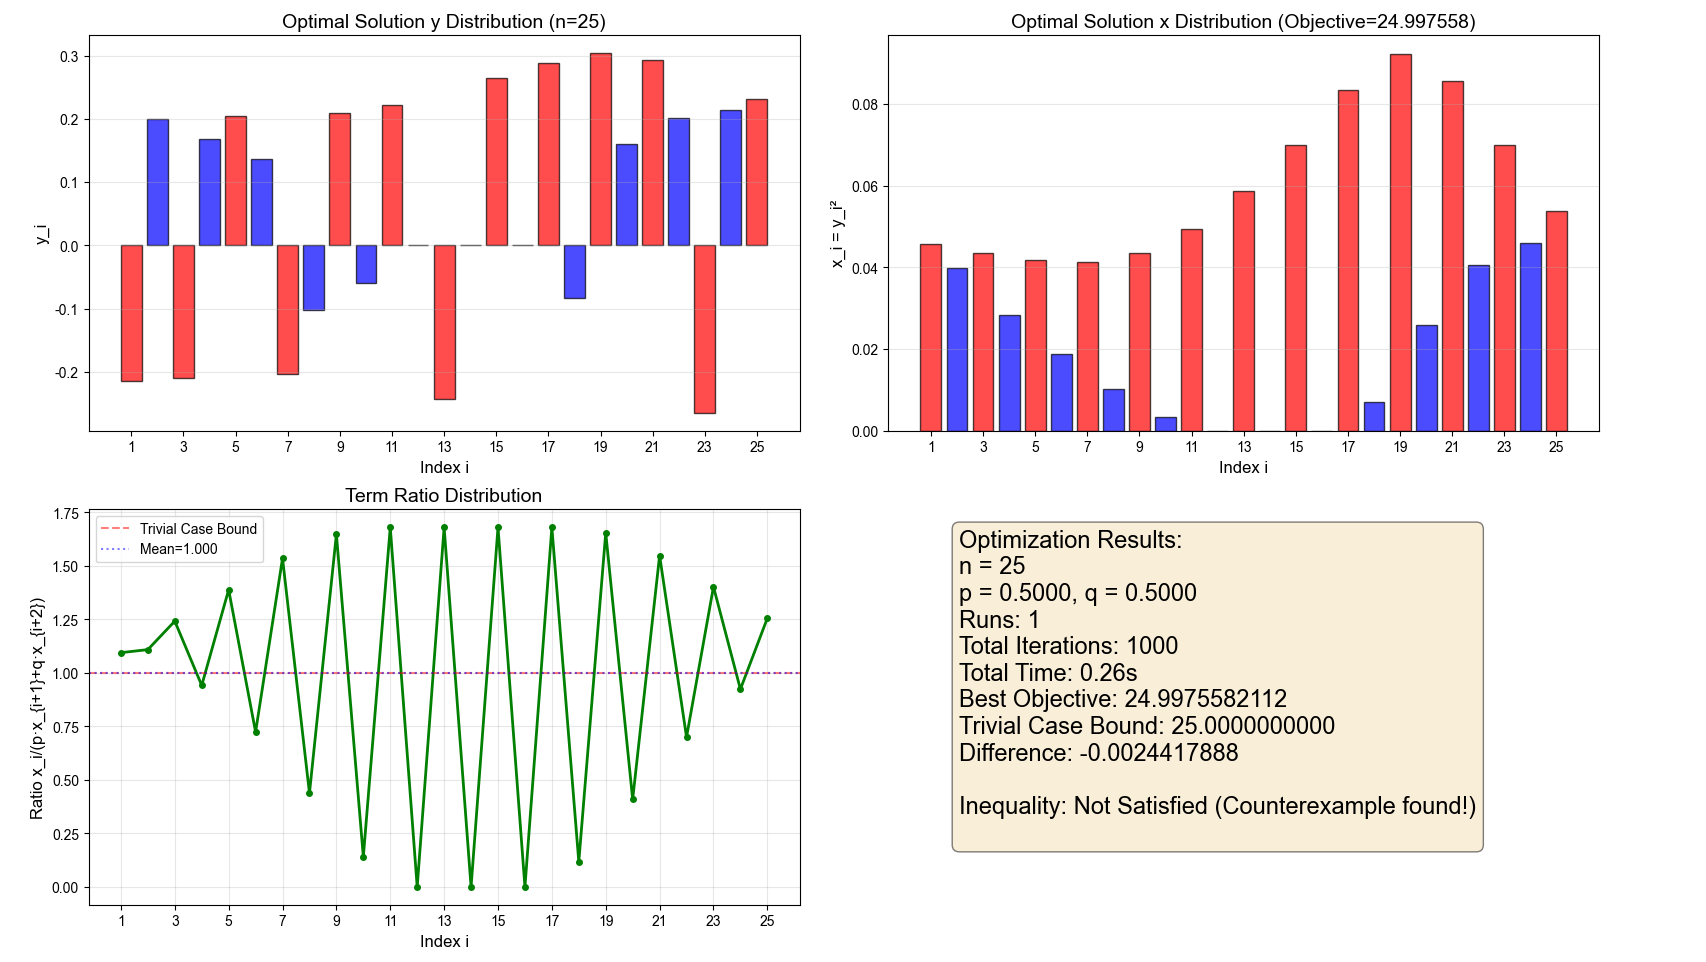
\includegraphics[width=0.55\linewidth]{figure/n=25,p=0.5_1}
%		\caption{Optimal Solution Distribution ($n=25, p=0.5$)}
%		\label{fig:n25p05_1}
%	\end{figure}
%	
%	\begin{figure}[!htbp]
%		\centering
%		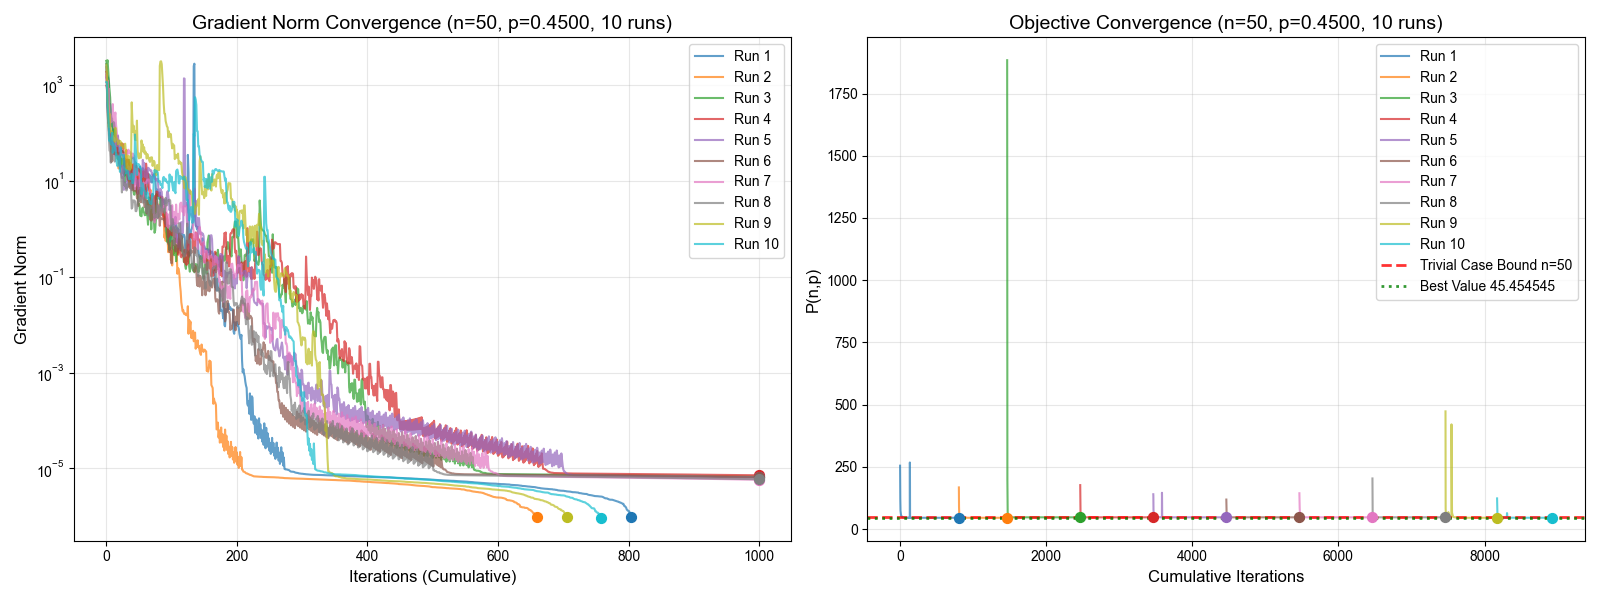
\includegraphics[width=0.55\linewidth]{figure/n=50,p=0.45}
%		\caption{Convergence of Shapiro Cyclic Sum and Gradient Norm ($n=50, p=0.45$)}
%		\label{fig:n50p45}
%	\end{figure}
%	
%	\begin{figure}[!htbp]
%		\centering
%		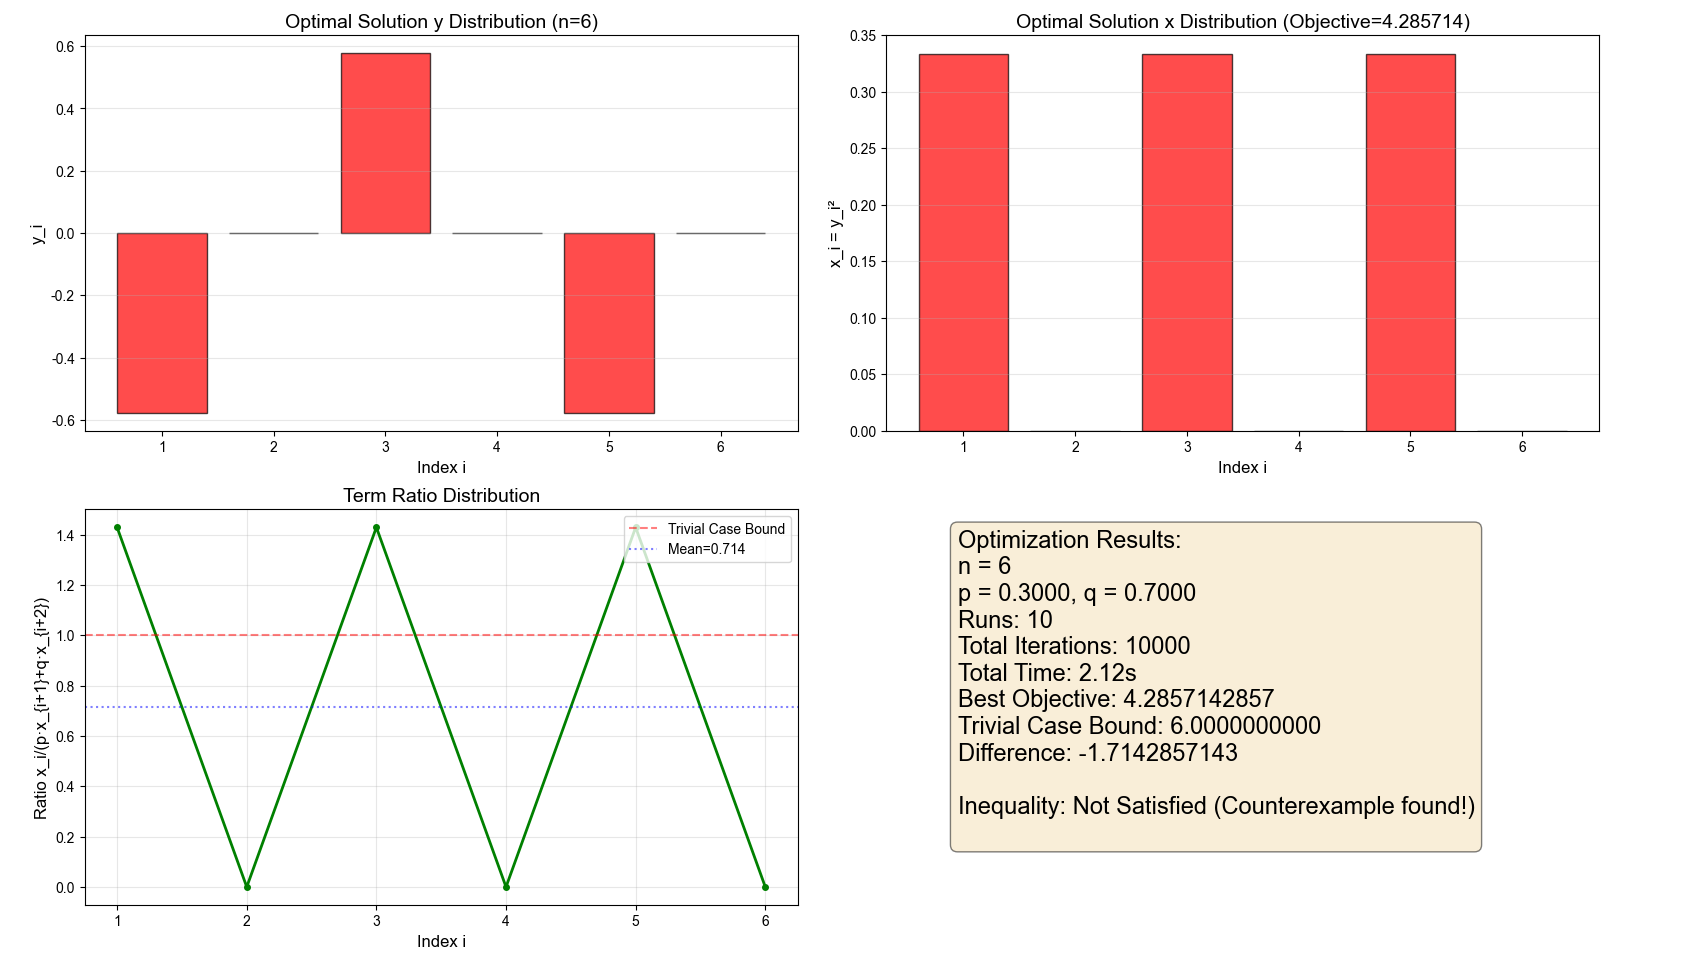
\includegraphics[width=0.55\linewidth]{figure/n=6,p=0.3_1}
%		\caption{Optimal Solution Distribution ($n=6, p=0.3$)}
%		\label{fig:n6p03_1}
%	\end{figure}
	
	\section{Acknowledgments}
	
	I would like to express my sincerest gratitude to my instructor in the Mathematical Analysis course and the supervisor of this research project, Professor Shengliang Pan. From the topic selection and literature review to the finalization of the paper, every step was accomplished under Professor Pan's meticulous guidance. It is a great fortune to have had the opportunity to complete this research under his supervision!
	
	I am also grateful to the School of Mathematical Sciences, Tongji University for providing a rich academic atmosphere. This work was supported by the Tongji University Student Innovation Training Program (SITP) under No. X2025634. I hereby express my sincere thanks.
	
	
	% Numbered list
	% Use the style of numbering in square brackets.
	% If nothing is used, default style will be taken.
	%\begin{enumerate}[a)]
	%\item 
	%\item 
	%\item 
	%\end{enumerate}  
	
	% Unnumbered list
	%\begin{itemize}
	%\item 
	%\item 
	%\item 
	%\end{itemize}  
	
	% Description list
	%\begin{description}
	%\item[]
	%\item[] 
	%\item[] 
	%\end{description}  
	
	%\clearpage %%Remove this from your manuscript
	
	
	% Figure
	%\begin{figure}%[]
	%\centering
	%    \includegraphics{}
	%\caption{}\label{fig1}
	%\end{figure}
	
	
	%\begin{table}%[]
	%\caption{}\label{tbl1}
	%\begin{tabular*}{\tblwidth}{@{}LL@{}}
	%\toprule
	
	%\midrule
	
	%\bottomrule
	%\end{tabular*}
	%\end{table}
	
	% Uncomment and use as the case may be
	%\begin{theorem} 
	%\end{theorem}
	
	% Uncomment and use as the case may be
	%\begin{lemma} 
	%\end{lemma}
	
	%% The Appendices part is started with the command \appendix;
	%% appendix sections are then done as normal sections
	%% \appendix
	
	%\section{}\label{}
	
	% To print the credit authorship contribution details
	%\printcredits
	
	%% Loading bibliography style file
	%\bibliographystyle{model1-num-names}
	%\bibliographystyle{cas-model2-names}
	%\bibliographystyle{elsarticle-num-names}
	\bibliographystyle{plainnat}
	
	% Loading bibliography database
	\bibliography{cas-refs}
	
	% Biography
	%\bio{}
	% Here goes the biography details.
	%\endbio
	
	%\bio{pic1}
	% Here goes the biography details.
	%\endbio
	
\end{document}

